\documentclass[aspectratio=169,11pt]{beamer}

% Shared style (ib-tutorials.sty at the repo root).
\makeatletter\def\input@path{{./}{../}}\makeatother
\usepackage{ib-tutorials}

\usepackage[utf8]{inputenc}
\usepackage{amsmath,amssymb}
\usepackage{booktabs}
\usepackage{array}
\newcolumntype{L}[1]{>{\raggedright\arraybackslash}p{#1}}
\usepackage{graphicx}
\graphicspath{{../pictures/4-ibfe/}{pictures/4-ibfe/}}
\usepackage{xcolor}
\usepackage{listings}
\usepackage{tikz}
\usetikzlibrary{arrows.meta,positioning,shapes.geometric,fit,calc,decorations.pathmorphing}
\usepackage{hyperref}

\newcommand{\sourcecredit}[1]{\vfill\begin{flushright}\tiny\textcolor{DarkGray}{#1}\end{flushright}}

\lstset{
  basicstyle=\ttfamily\scriptsize\color{BlackGray},
  keywordstyle=\color{NavyBlue}\bfseries,
  commentstyle=\color{DarkGray}\itshape,
  stringstyle=\color{OliveGreen},
  showstringspaces=false,
  columns=fullflexible,
  keepspaces=true,
  breaklines=true,
  breakindent=1em,
  frame=single,
  framerule=0.4pt,
  rulecolor=\color{LightGray},
  backgroundcolor=\color{LightGray!30},
  xleftmargin=0.25em,
  xrightmargin=0.25em
}
\lstdefinestyle{shell}{morecomment=[l]{\#}}
\lstdefinestyle{input}{morecomment=[l]{//}}
\lstdefinestyle{matlab}{morecomment=[l]{\%}}
\lstdefinestyle{python}{morecomment=[l]{\#}}
\lstdefinestyle{data}{}
\lstdefinestyle{tiny}{basicstyle=\ttfamily\tiny\color{BlackGray}}
\lstdefinestyle{inputtiny}{morecomment=[l]{//},basicstyle=\ttfamily\tiny\color{BlackGray}}
\lstdefinestyle{matlabtiny}{morecomment=[l]{\%},basicstyle=\ttfamily\tiny\color{BlackGray}}
\lstdefinestyle{pythontiny}{morecomment=[l]{\#},basicstyle=\ttfamily\tiny\color{BlackGray}}
\lstdefinestyle{cpp}{language=C++,morecomment=[l]{//}}
\lstdefinestyle{cpptiny}{language=C++,morecomment=[l]{//},basicstyle=\ttfamily\tiny\color{BlackGray}}
\lstdefinestyle{cmake}{morecomment=[l]{\#}}
\lstdefinestyle{geo}{morecomment=[l]{//}}
\lstdefinestyle{geotiny}{morecomment=[l]{//},basicstyle=\ttfamily\tiny\color{BlackGray}}
\lstdefinestyle{datatiny}{basicstyle=\ttfamily\tiny\color{BlackGray}}

\title[Creating meshes]{Creating meshes}
\subtitle{gmsh by script and by mouse, Triangle and TetGen from \code{.poly} files, CAD to Coreform Cubit to ExodusII, libMesh's own generators, and the element-size rules reconciled}
\author[Miller]{Laura A. Miller}
\institute[UArizona]{Department of Mathematics, University of Arizona}
\date{Using IB Software \textbullet\ Part IV \textbullet\ Chapter 18}

\begin{document}

% 1
\begin{frame}[plain]
\maketutorialtitlepanel{%
\begin{tikzpicture}[scale=0.84]
  % a triangle meshed with triangles
  \coordinate (A) at (0.3,0.3); \coordinate (B) at (2.1,0.3); \coordinate (C) at (0.3,2.1);
  \foreach \i in {1,2,3,4,5} {
    \draw[BlackGray,thin] ($(A)!\i/6!(B)$) -- ($(A)!\i/6!(C)$);
    \draw[BlackGray,thin] ($(A)!\i/6!(B)$) -- ($(B)!\i/6!(C)$);
    \draw[BlackGray,thin] ($(A)!\i/6!(C)$) -- ($(C)!\i/6!(B)$);
  }
  \draw[NavyBlue,thick] (A) -- (B) -- (C) -- cycle;
  \node[font=\tiny,text=NavyBlue] at (1.6,1.6) {\code{Physical Surface}};
  % a hex tube
  \foreach \k in {0,...,6} \draw[OliveGreen,thin] (2.6+0.22*\k,0.5) ellipse (0.08 and 0.3);
  \draw[OliveGreen,thick] (2.6,0.8) -- (3.92,0.8); \draw[OliveGreen,thick] (2.6,0.2) -- (3.92,0.2);
  \node[font=\tiny,text=OliveGreen] at (3.3,1.2) {\code{Transfinite}, \code{Recombine}};
  \node[font=\tiny,text=RubineRed] at (3.2,2.0) {\code{gmsh -2 -format msh22}};
  \node[font=\tiny,text=DarkGray] at (3.2,1.65) {\code{.msh} \textbullet\ \code{.node/.ele} \textbullet\ \code{.e} \textbullet\ \code{.mat}};
\end{tikzpicture}}
\end{frame}

% 2
\begin{frame}{Learning goals}
\label{fr:goals}
\footnotesize By the end of this chapter you should be able to:
\begin{enumerate}
  \item say what a mesh must have before IBFE will take it: the right dimension, an element type libMesh knows, elements that go round the right way, a size that fits the fluid grid, and a file format with an extension libMesh recognises;
  \item make a 2D mesh with gmsh three ways, by script, by mouse and by command line, and export it in a version libMesh reads;
  \item make a 3D mesh with gmsh from a \code{.geo} file (extrusion, revolution, a transfinite hex tube), and finish Nick Battista's 2014 tube tutorial, which stopped at a surface;
  \item write a \code{.poly} file and mesh it with Triangle (2D) or TetGen (3D), including holes, and read the result;
  \item take a CAD model through Coreform Cubit (once Trelis and Bolt) to an ExodusII file whose blocks become libMesh subdomains;
  \item build a mesh inside the program with libMesh's generators, as IBAMR's own examples do;
  \item choose an element size: the five rules the course taught over ten years, what IBAMR actually does with the mesh, and the rule that follows;
  \item recognise the errors a bad mesh produces (\code{Jacobian ... must be positive}, \code{mesh\_dimension() == spatial\_dimension()}, \code{Unknown data format}, \code{Unrecognized file extension}) and fix the file.
\end{enumerate}
\end{frame}

% 3
\begin{frame}{Where this chapter comes from}
\label{fr:sources}
\scriptsize
\begin{itemize}
  \item \al{Alex Hoover, ``2-IBFE Tutorial: Creating your mesh'' (2014--2017, 11 slides):} element types, the four parts of a \code{.poly} file, TetGen and \code{TetGenIO}. Two of its slides, \emph{Holes} and \emph{Generating your elements}, were never written (slides \ref{fr:holes} and \ref{fr:tetgenrun} write them), and its element-type list had names that do not exist (slide \ref{fr:elemtypes}).
  \item \al{``2.1 - IBFE Tutorial: Make your own mesh and move it!'' (Feb 2017; MATH 769 2018; lab versions 2020 and 2024-08-01, 16 slides):} the gmsh GUI homework: a triangle with legs $0.5$, meshed at the fine grid spacing, swapped into the plate example with \code{MFAC = 1} and \code{IB\_POINT\_DENSITY = 1}. Example IBFE/05 is this homework, done.
  \item \al{Julian Wag, ``Using gmsh to make 2D meshes from scratch'' (2016, 13 slides with GUI screenshots):} points, lines, plane surface, Mesh 2D, the global mesh size factor, Save as \code{.msh}. Five of its screenshots are reproduced here with credit.
  \item \al{Nick Battista, ``How To Make Simple Geometries in Gmsh'' (24 September 2014, 11 pages):} a tube from parameters, points at the ``poles'', circle arcs, line segments, ruled and plane surfaces; it ends at a surface mesh. The PDF is in every copy of the course folders; its 46 screenshots are not reproduced (slides \ref{fr:battista} and \ref{fr:battista2} transcribe the steps).
  \item \al{The meshing read-mes (2015--2017):} the gmsh links and the sizing rule (``average size should equal Cartesian mesh width''), the Trelis read-me (a shared floating licence; csimsoft tutorials), the 2016 Trelis notes (pave then sweep, merge, wall thickness, 1:1), and the vendor's \emph{Getting Started with Trelis} PDF (2014, linked, not reproduced). The meshing read-me's forwarded IT e-mail and licence host are not reproduced.
  \item \al{The 2020 ``Plans for June'' deck:} the tool list (gmsh, Trelis, Bolt, Meshmixer); the CAD route of the two-coral example (chapter 21).
  \item \al{New here:} every command of this chapter was run with gmsh 4.12.1, Triangle and TetGen (slide \ref{fr:run}); the MSH 2.2 / 4.1 / binary question; the two rules a gmsh file must obey; what gmsh physical groups and Exodus blocks become in libMesh; the generators of IBAMR's own examples; the element-size rules reconciled from the upstream inputs.
\end{itemize}
\end{frame}

% 4
\begin{frame}{What a mesh must have before IBFE will take it}
\label{fr:musthave}
\scriptsize
\vspace{-6pt}
\begin{tabular}{@{}L{0.20\textwidth}L{0.72\textwidth}@{}}
\toprule
property & what IBFE needs \\
\midrule
dimension & the mesh dimension equals the program's: triangles or quadrilaterals for \code{main2d}, tetrahedra or hexahedra for \code{main3d}. A file that holds only lines (or only surface triangles in 3D) fails with \code{Failed assertion: mesh->mesh\_dimension() == mesh->spatial\_dimension()}. \\
element type & one of libMesh's (slide \ref{fr:elemtypes}); the type is in the file (gmsh, Exodus, TetGen) or given when the mesh is built (\code{ELEM\_TYPE}). \\
orientation & every element's nodes must go round so that its Jacobian is positive; IBAMR checks and stops otherwise (slide \ref{fr:tworules}). \\
size and position & in the simulation's units, already placed where it belongs in the box (or moved by an initial coordinate mapping, chapter 22); an element size matched to the fine grid spacing (slide \ref{fr:rules}). \\
one file, one extension & the extension picks the reader (chapter 17, slide 32): \code{.msh} gmsh ASCII, \code{.e} or \code{.exo} ExodusII, \code{.node} and \code{.ele} TetGen, \code{.mat} MATLAB, \code{.inp} Abaqus, \code{.vtu}, \code{.unv}, \code{.ucd}, \code{.off}, \code{.mesh}, \code{.xda} or \code{.xdr}, \code{.cpa} or \code{.cpr}. Nothing else is recognised. \\
groups (optional) & gmsh physical groups and Exodus blocks become libMesh subdomain ids and names; lower-dimensional groups become side sets; chapter 21 uses them to give parts of one mesh different materials. \\
\bottomrule
\end{tabular}

\begin{punchbox}
\scriptsize ``In keeping with the practice of using \code{.vertex}, \code{.spring} and \code{.beam} files for complicated geometries, this tutorial is focused on the TetGen, Triangle and MATLAB tools'' (2014). Ten years on, gmsh covers most of it, and Coreform Cubit the CAD end.
\end{punchbox}
\end{frame}

% 5
\begin{frame}{Element types: libMesh's names, gmsh's numbers, and the 2014 slide's slips}
\label{fr:elemtypes}
\scriptsize
\begin{tabular}{@{}llllL{0.40\textwidth}@{}}
\toprule
dimension & libMesh type & nodes & gmsh type & notes \\
\midrule
2D & \code{TRI3} & 3 & 2 & linear triangle; the course's meshes (IBFE/01, 05, 06, 08, 12) \\
   & \code{TRI6} & 6 & 9 & quadratic triangle; upstream ex4, ex5 \\
   & \code{QUAD4} & 4 & 3 & bilinear quadrilateral \\
   & \code{QUAD8}, \code{QUAD9} & 8, 9 & 16, 10 & quadratic quadrilaterals; \code{QUAD9} in upstream ex0--ex3, ex9 \\
3D & \code{TET4} & 4 & 4 & linear tetrahedron; gmsh's default in 3D, TetGen's output, IBFE/10 \\
   & \code{TET10} & 10 & 11 & quadratic tetrahedron \\
   & \code{HEX8} & 8 & 5 & trilinear hexahedron; upstream ex2 and ex4 in 3D \\
   & \code{HEX20}, \code{HEX27} & 20, 27 & 17, 12 & quadratic hexahedra; \code{HEX27} in upstream ex5 and ex9 in 3D \\
   & \code{PRISM6}, \code{PRISM15}, \code{PRISM18} & 6, 15, 18 & 6, 18, 13 & wedges \\
   & \code{PYRAMID5} & 5 & 7 & pyramids \\
\bottomrule
\end{tabular}

\end{frame}

% 5b
\begin{frame}{Element types (2): what the table says, and the 2014 slide's slips}
\label{fr:elemtypes2}
\footnotesize
\begin{itemize}
  \item The gmsh numbers are the ones libMesh's \code{GmshIO} maps (\code{gmsh\_io.C}, the \code{ElementDefinition} table); a gmsh type outside this list stops the read.
  \item The 2014 slide listed ``\code{TET4}, \code{TET8}'' and ``Hexagonal (\code{HEX6}, \code{HEX8})''. There is no \code{TET8} (it is \code{TET10}) and no \code{HEX6} (a six-node element is a prism); ``hexagonal'' should be \emph{hexahedral}.
  \item ``Piecewise linear or piecewise cubic'' (2014): the choice is linear (\code{TRI3}, \code{QUAD4}, \code{TET4}, \code{HEX8}) or quadratic (the rest); libMesh has no cubic Lagrange elements in this family.
  \item A \code{MATLAB .mat} file is triangles only; TetGen writes \code{TET4} only; Triangle writes \code{TRI3} (or 6-node triangles with \code{-o2}, which libMesh's TetGen reader does not take); gmsh and Cubit write any of these.
\end{itemize}
\end{frame}

% 6
\begin{frame}{What IBAMR's own examples use}
\label{fr:upstream}
\scriptsize
Every upstream IBFE example builds its mesh in the program (slide \ref{fr:generators}) with an element size \code{ds = MFAC*DX}; these are their input files in 0.19.0:

\setlength{\tabcolsep}{3pt}
\begin{tabular}{@{}L{0.13\textwidth}L{0.15\textwidth}L{0.07\textwidth}L{0.10\textwidth}L{0.19\textwidth}L{0.24\textwidth}@{}}
\toprule
example & \code{ELEM\_TYPE} & \code{MFAC} & \code{IB\_POINT\_} \code{DENSITY} & \code{PK1\_DEV} / \code{DIL\_QUAD\_ORDER} & what it is \\
\midrule
ex0, ex1 (2D) & \code{QUAD9} & 4.0 & 2.0 & -- & a rubber band (thin ring), stretched band \\
ex2 (2D / 3D) & \code{QUAD9} / \code{HEX8} & 2.0 & 2.0 & FIFTH/THIRD, THIRD/FIRST & an elastic block in a channel \\
ex3 (2D) & \code{QUAD9} & 2.0 & 2.0 & FIFTH/THIRD & a block with a different stress \\
ex4 (2D / 3D) & \code{TRI6} / \code{HEX8} & 2.0 / 1.0 & 3.0 & FIFTH/THIRD, THIRD/FIRST & a compressible disc / sphere \\
ex5 (2D / 3D) & \code{TRI6} / \code{HEX27} & 8.0 & 4.0 & SEVENTH/FIFTH & a disc / sphere in a stream \\
ex6 (2D) & (input) & 1.0 & 1.0 & -- & a disc and a beam (two parts) \\
ex8 (2D) & (input) & -- & 2.0 & FIFTH/THIRD & three parts \\
ex9 (2D / 3D) & \code{QUAD9} / \code{HEX27} & 4.0 / 8.0 & 4.0 & SEVENTH/FIFTH & a thin shell \\
ex10, ex11 (2D) & \code{TRI3} & 2.0 / 8.0 & 4.0 & -- & direct-forcing rigid bodies \\
\bottomrule
\end{tabular}

\medskip
\begin{itemize}
  \item \code{MFAC} runs from $1$ to $8$ and \code{IB\_POINT\_DENSITY} from $1$ to $4$: elements up to eight grid cells wide work when the quadrature puts enough points in each cell. That is the key to slide \ref{fr:rules}.
  \item Quadratic elements (\code{QUAD9}, \code{TRI6}, \code{HEX27}) carry the larger \code{MFAC}; linear ones (\code{TRI3}, \code{HEX8}) sit at $1$--$2$.
  \item The course's examples read their meshes from files, so their \code{MFAC} lines do nothing (chapter 17); their element sizes were chosen when the files were made: $2\,\mathrm{DX}$ for IBFE/01, $1\,\mathrm{DX}$ for IBFE/05, about $3\,\mathrm{DX}$ for IBFE/10's plate.
\end{itemize}
\end{frame}

% 7
\begin{frame}{Five routes to a mesh}
\label{fr:routes}
\scriptsize
\begin{tabular}{@{}L{0.18\textwidth}L{0.30\textwidth}L{0.22\textwidth}L{0.20\textwidth}@{}}
\toprule
route & tools & output & used by \\
\midrule
A. build it in the program & libMesh \code{MeshTools::Generation} (\code{build\_square}, \code{build\_cube}, \code{build\_sphere}) & none: the mesh exists in memory & every upstream IBFE example (slide \ref{fr:generators}) \\
B. gmsh & a \code{.geo} script or the GUI; \code{gmsh -2}/\code{-3} & \code{.msh} (ASCII 2.2 or 4.1) & IBFE/05 (2D), IBFE/10 (3D); chapters 21, 22 \\
C. Triangle / TetGen & a \code{.poly} file; \code{triangle -pq}, \code{tetgen -pq} & \code{.node} + \code{.ele} (+ \code{.face}, \code{.edge}) & the 2014 tutorial; the course's \code{Beam\_IBFE\_Mesh2D.m} \\
D. CAD to a mesher & Fusion 360, SolidWorks, Blender, SpaceClaim $\to$ STEP or STL $\to$ Coreform Cubit (or gmsh) & \code{.e} ExodusII (or \code{.msh}) & IBFE/08 (Trelis); the two corals (chapter 21); the carotid artery (coming) \\
E. MATLAB PDE Toolbox & \code{pdepoly}, \code{initmesh}, a \code{fprintf} loop & \code{.mat} (triangles) & IBFE/01, 06, 12 (chapter 17, slide 39) \\
\bottomrule
\end{tabular}

\end{frame}

% 7b
\begin{frame}{Five routes to a mesh (2): which to learn}
\label{fr:routes2}
\footnotesize
\begin{itemize}
  \item Route A needs no file and no other program; it makes rectangles, boxes, discs and spheres, and anything you can deform them into with a loop over the nodes (ex6 shifts a disc by $0.2$ that way).
  \item Routes B and C are free and scriptable; B is the one to learn.
  \item Route D is for shapes that start as CAD: scans, drawings, bodies with fillets and holes. Cubit also makes hexahedral meshes, which gmsh does only for simple shapes.
  \item Whatever the route, the file goes through \code{mesh.read()} and the checks of slide \ref{fr:checks}.
\end{itemize}
\end{frame}

% 8
\begin{frame}[fragile]{Route A: libMesh's generators, as IBAMR's examples use them}
\label{fr:generators}
\footnotesize
Upstream \code{IBFE/explicit/ex2} (an elastic block $0.1$ wide and $1$ tall, at $0.95 < x < 1.05$):
\begin{lstlisting}[style=cpptiny]
Mesh mesh(init.comm(), NDIM);
const double dx = input_db->getDouble("DX");
const double ds = input_db->getDouble("MFAC") * dx;            // the element size: MFAC fine-grid cells
string elem_type = input_db->getString("ELEM_TYPE");
#if (NDIM == 2)
MeshTools::Generation::build_square(mesh,
                                    static_cast<int>(ceil(0.1 / ds)),   // elements across
                                    static_cast<int>(ceil(1.0 / ds)),   // elements up
                                    0.95, 1.05,                         // xmin, xmax
                                    0.0, 1,                             // ymin, ymax
                                    Utility::string_to_enum<ElemType>(elem_type));
#endif
#if (NDIM == 3)
MeshTools::Generation::build_cube(mesh,
                                  static_cast<int>(ceil(0.1 / ds)), static_cast<int>(ceil(1.0 / ds)), static_cast<int>(ceil(1.0 / ds)),
                                  0.95, 1.05, 0.0, 1, 0.0, 1,
                                  Utility::string_to_enum<ElemType>(elem_type));
#endif
\end{lstlisting}
\begin{itemize}
  \item \code{nx}, \code{ny} (\code{nz}) are element counts, so \code{ceil(length / ds)} turns a size into a count; the element type comes from the input as a string, through \code{Utility::string\_to\_enum<ElemType>}.
\end{itemize}
\end{frame}

% 8b
\begin{frame}[fragile]{Route A (2): the generators' signatures, and placing the result}
\label{fr:generators2}
\footnotesize
The signatures (libMesh 1.7.8, \code{mesh\_generation.h}):
\begin{lstlisting}[style=cpptiny]
void build_square(UnstructuredMesh& mesh, unsigned int nx, unsigned int ny, Real xmin = 0., Real xmax = 1., Real ymin = 0., Real ymax = 1., ElemType type = INVALID_ELEM, bool gauss_lobatto_grid = false);
void build_cube(UnstructuredMesh& mesh, unsigned int nx = 0, unsigned int ny = 0, unsigned int nz = 0, Real xmin = 0., Real xmax = 1., Real ymin = 0., Real ymax = 1., Real zmin = 0., Real zmax = 1., ElemType type = INVALID_ELEM, bool gauss_lobatto_grid = false);
void build_sphere(UnstructuredMesh& mesh, Real rad = 1, unsigned int nr = 2, ElemType type = INVALID_ELEM, unsigned int n_smooth = 2, bool flat = true);
\end{lstlisting}
\begin{itemize}
  \item \code{build\_sphere} makes a disc in 2D and a ball in 3D with $4\cdot 2^{r}$ segments around; ex6 chooses $r$ from \code{ds}: \code{num\_circum\_segments = ceil(2 pi R / ds); r = log2(0.25 * num\_circum\_segments)}, then shifts every node by $(0.2, 0.2)$ in a loop over \code{block\_mesh.nodes\_begin()}. That loop is the generator route's answer to ``how do I place it?''.
  \item Boundary ids are set to the side indexing of the master element (``\code{build\_square}: boundary ids are set to be equal to the side indexing on a master quad''), which ex2 then relabels in a loop over the elements' sides.
\end{itemize}
\end{frame}

% 9
\begin{frame}[fragile]{Route B: gmsh in one slide}
\label{fr:gmshbasics}
\footnotesize
gmsh (\url{https://gmsh.info}, open source) builds geometry from points, curves, surfaces and volumes, in a text file (\code{.geo}) or by mouse, and meshes it. The pieces of a \code{.geo} file:
\begin{lstlisting}[style=geotiny]
lc = 0.0156;                                  // a variable: the target element size
Point(1) = {0.5, 0.0, 0.0, lc};               // x, y, z, element size at the point
Line(1) = {3, 2};                             // a straight line between two points
Circle(1) = {2, 1, 3};                        // an arc: start point, centre, end point (less than a half turn)
Curve Loop(4) = {1, 2, -3};                   // a closed loop of curves, minus = reversed ("Line Loop" in gmsh 2 and 3)
Plane Surface(5) = {4};                       // a flat surface bounded by the loop (holes: more loops)
Surface(14) = {13};                           // a curved surface ("Ruled Surface" in gmsh 2 and 3)
Surface Loop(29) = {28, 26, 16, 14};          // a closed shell of surfaces
Volume(30) = {29};                            // the solid inside it
Extrude {0, 0, 1} { Surface{6}; }             // sweep a surface into a volume (translation)
Extrude {{0,0,1}, {0,0,0}, Pi/2} { Surface{5}; }   // revolve a surface about an axis
Physical Surface("triangle", 1) = {5};        // the group the mesh file will keep (2D)
Physical Volume("tube") = {179, 181};         // the same in 3D
Transfinite Line {1, 2} = 24; Transfinite Surface "*"; Recombine Surface "*"; Transfinite Volume "*";   // a structured hex mesh
Mesh.Algorithm = 5;                           // 2D algorithm: 5 Delaunay, 6 Frontal-Delaunay (gmsh 4's default)
\end{lstlisting}
\begin{itemize}
  \item Every entity has a number; the numbers are shared across curve types (``even though it says \code{Line(12)}, we have only defined 4 lines so far'': Battista), so take the next free one or let the GUI do it.
  \item A \code{.geo} file is reloaded with \textbf{Reload} after every edit; the GUI writes the same commands into the file when you click, so you can mix the two (Battista's method, slide \ref{fr:battista}).
  \item The file's element size is \code{lc} at the points, scaled by \textbf{Global mesh size factor} (\code{Mesh.MeshSizeFactor}, slide \ref{fr:wag2}).
\end{itemize}
\end{frame}

% 10
\begin{frame}[fragile]{The triangle of IBFE/05: \code{triangle.geo}}
\label{fr:trianglegeo}
\footnotesize
\begin{columns}[T]
\column{0.58\textwidth}
\begin{lstlisting}[style=geotiny]
// triangle.geo: gmsh script for the triangle of example IBFE/05.
// Make a mesh file that libMesh can read (ASCII text, MSH format 2.2):
//   gmsh -2 -format msh22 triangle.geo -o triangle_gmsh.msh
// libMesh reads ASCII MSH files (format 2.2 or 4.1) but not binary ones.

// Target element size: about one finest grid cell, DX = L/NFINEST = 2/128.
lc = 0.0156;
// 2D meshing algorithm: 5 is Delaunay. With it, gmsh 4.12 makes the same
// numbers of nodes and triangles as the course mesh (759 and 1404). Without
// this line gmsh 4 uses Frontal-Delaunay (6): 687 nodes and 1260 triangles.
Mesh.Algorithm = 5;

Point(1) = {0.5, 0.0, 0.0, lc};
Point(2) = {0.0, 0.0, 0.0, lc};
Point(3) = {0.0, 0.5, 0.0, lc};

Line(1) = {3, 2};          // left side, on x = 0
Line(2) = {2, 1};          // bottom side, on y = 0
Line(3) = {3, 1};          // the long side

Curve Loop(4) = {1, 2, -3};  // "Line Loop" in gmsh 3 and older
Plane Surface(5) = {4};

// Once a file has any physical group, gmsh saves only the elements that
// belong to a physical group. A 2D mesh therefore needs a Physical Surface.
Physical Surface("triangle", 1) = {5};
\end{lstlisting}
\column{0.40\textwidth}
\scriptsize Twenty lines: a size, an algorithm, three points, three lines, a loop, a surface, a group. The comments are the file's own; they record what was found when the course's \code{triangle.msh} was reproduced (next slide).
\end{columns}
\end{frame}

% 10b
\begin{frame}{The triangle of IBFE/05 (2): what the script makes}
\label{fr:trianglegeo2}
\begin{columns}[T]
\column{0.42\textwidth}
\begin{center}
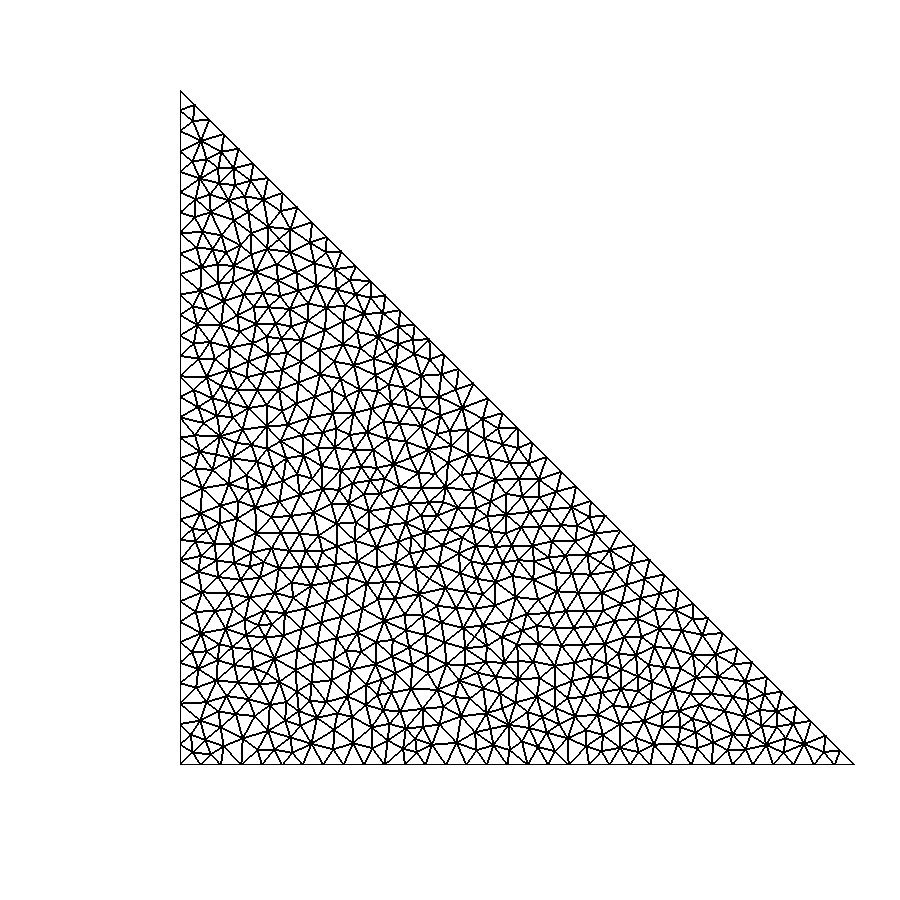
\includegraphics[width=\textwidth]{ch18-triangle-gmsh.png}
\end{center}
\column{0.56\textwidth}
\footnotesize The 2017 homework's triangle, ``corners $(0.5, 0)$, $(0, 0)$ and $(0, 0.5)$'' (``Remember you want to select these so they will fit in your domain'': $L = 2$, from $-1$ to $1$), meshed at the fine grid spacing: $759$ nodes, $1404$ triangles, the same counts as the course's \code{triangle.msh}. ``We want the ratio of the finite element mesh to the Cartesian mesh to be 1:1. We will therefore pick a meshwidth of $L/\mathrm{NFINEST} = 2.0/128 = 0.0156$.''
\end{columns}
\end{frame}

% 11
\begin{frame}[fragile]{Running gmsh from the command line, and which MSH version to write}
\label{fr:mshversions}
\footnotesize
\begin{lstlisting}[style=shell]
gmsh -2 -format msh22 triangle.geo -o triangle.msh     # 2D mesh, MSH 2.2 ASCII
gmsh -3 -format msh22 cube.geo -o cube.msh             # 3D mesh
gmsh -2 triangle.geo -o triangle41.msh                 # gmsh 4's default: MSH 4.1 ASCII (libMesh reads it too)
gmsh -2 -format msh22 -bin triangle.geo -o bad.msh     # binary: libMesh cannot read it
gmsh tube.geo -0 -format msh22                         # run a script that meshes and saves itself ("Mesh 3; Save ...")
gmsh plate2.msh -save -format vtk -o plate2.vtk        # convert a mesh (here for VisIt)
\end{lstlisting}
\begin{tabular}{@{}L{0.22\textwidth}L{0.70\textwidth}@{}}
\toprule
format & libMesh 1.7.8 \\
\midrule
MSH 2.2 ASCII & read and written; the safe choice; what every example here ships (\code{\$MeshFormat} line: \code{2.2 0 8}) \\
MSH 4.0, 4.1 ASCII & read since libMesh 1.5 (``Mesh version 4.0 is a near complete rewrite''); gmsh 4 writes 4.1 unless told otherwise (\code{4.1 0 8}) \\
MSH 1.0 & read (``\code{version <= 1.0}'' branch) \\
any binary MSH & not read: \code{Error: Unknown data format for mesh in Gmsh reader.} (\code{2.2 1 8}: the middle 1 means binary) \\
\bottomrule
\end{tabular}

\end{frame}

% 11b
\begin{frame}{MSH versions (2): the GUI's export dialog, and ``version ???''}
\label{fr:mshversions2}
\footnotesize
\begin{itemize}
  \item In the GUI: \textbf{File $\to$ Export}, choose \emph{Mesh - Gmsh MSH (*.msh)}, and in the dialog pick \emph{Version 2 ASCII} (the 2017 slide's ``choose the .msh file type in the drop down list'' predates the version dialog; Wag's 2016 slide used \emph{Save as}).
  \item The 2020 and 2024 decks say ``Download gmsh, version ???; we previously used 2.9.0.'' Any gmsh 4 works; the syntax changes are the names in slide \ref{fr:gmshbasics}, which gmsh 4.12 still accepts.
\end{itemize}
\end{frame}

% 12
\begin{frame}[fragile]{The two rules a gmsh file must obey, and the errors when it does not}
\label{fr:tworules}
\scriptsize
\begin{enumerate}
  \item \al{Go round the surface counter-clockwise.} gmsh numbers each triangle's corners in the direction of the curve loop. A clockwise loop (\code{\{3, -2, -1\}} for the triangle) makes every triangle clockwise, and IBAMR stops at start-up:
\begin{lstlisting}[style=datatiny]
IBAMR requires that the Jacobian of each element must be positive, but the present element has at least one point at which the Jacobian is either negative or zero.
... (the element's corners) ...
To get around this error, you will need to edit the problematic mesh either by hand or with a CAD program.
\end{lstlisting}
  Fixes: reverse the loop; \code{ReverseMesh Surface\{5\};} in the \code{.geo}; or \code{python3 fix\_orientation.py old.msh new.msh} (IBFE/05 ships it: it swaps the last two nodes of every clockwise triangle and changes nothing else). The course's \code{triangle.msh} had all $1404$ triangles clockwise; IBAMR has checked since 0.11.0 (2022).
  \item \al{Put the surface (or volume) in a physical group.} Once a file has any physical group, gmsh saves only elements in physical groups. A file with only a \code{Physical Curve} holds the $112$ boundary lines and no triangles, and the mesh is one-dimensional:
\begin{lstlisting}[style=datatiny]
Failed assertion: mesh->mesh_dimension() == mesh->spatial_dimension()
\end{lstlisting}
  With no physical group at all, gmsh saves everything, including the points and lines (slide \ref{fr:samples}); libMesh turns the lower-dimensional elements into boundary information, so this also works, but the file is bigger.
\end{enumerate}
All three cases of this slide were run with IBAMR 0.16.0 and 0.19.0 (IBFE/05's README) and give these messages.
\end{frame}

% 13
\begin{frame}{The GUI route (1): points, lines, a plane surface}
\label{fr:wag1}
\footnotesize
\begin{columns}[T]
\column{0.5\textwidth}
Julian Wag's 2016 steps, kept by the 2017--2024 homework decks:
\begin{enumerate}
  \item \textbf{Modules $\to$ Geometry $\to$ Elementary entities $\to$ Add $\to$ Point}: type the coordinates, or place the point with the mouse and press \textbf{e}; \textbf{q} ends the mode. ``If using the mouse, change the snap value for more or less precision.'' Set \emph{Prescribed mesh element size at point} to the element size ($0.0156$ in the homework).
  \item \textbf{Add $\to$ Straight line} (or Spline, Circle arc): click the two end points of each line.
  \item \textbf{Add $\to$ Plane surface}: click the closed border and press \textbf{e}; ``the plane is indicated by dashed lines in the middle of the border lines.''
\end{enumerate}
\column{0.48\textwidth}
\begin{center}
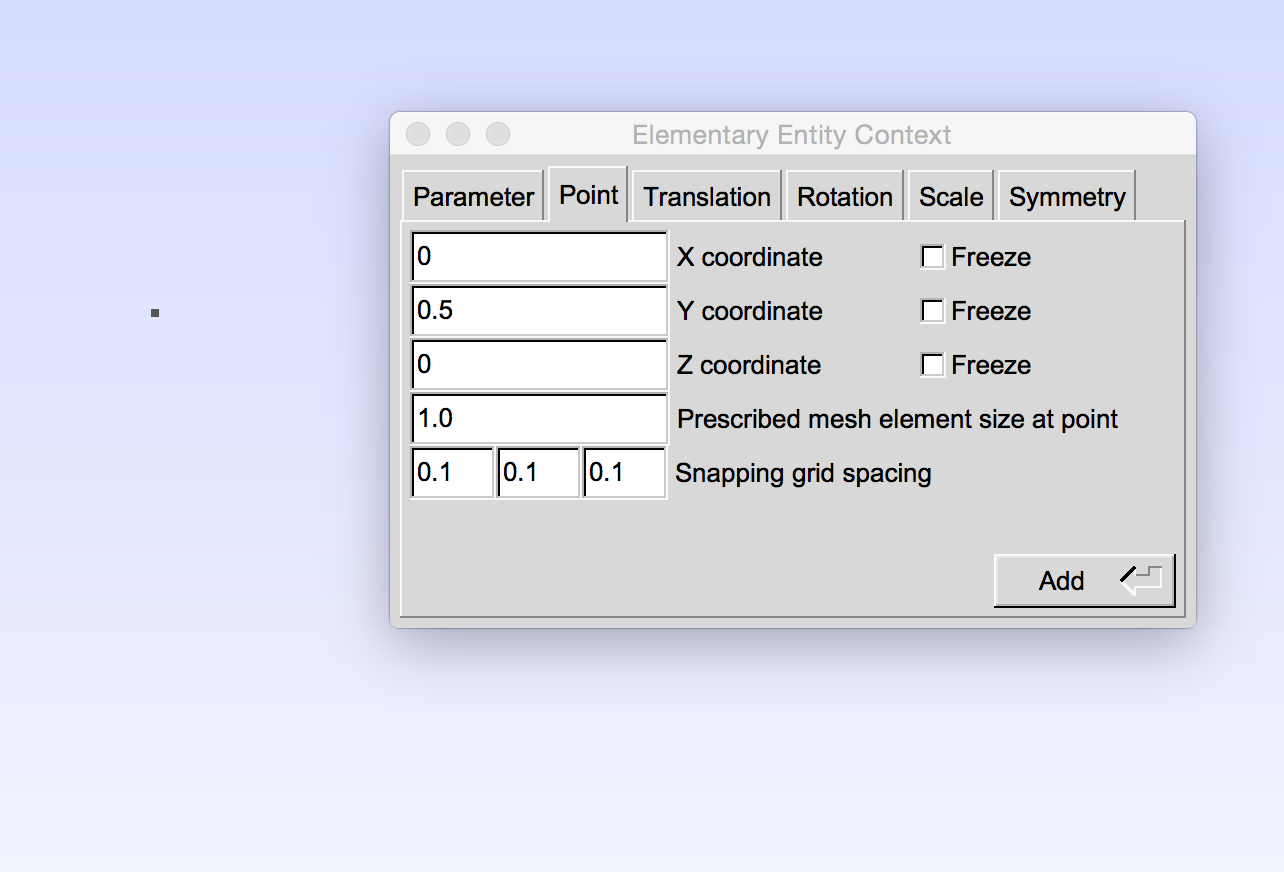
\includegraphics[height=0.36\textheight]{ch18-wag-addpoint.png}\\[2pt]
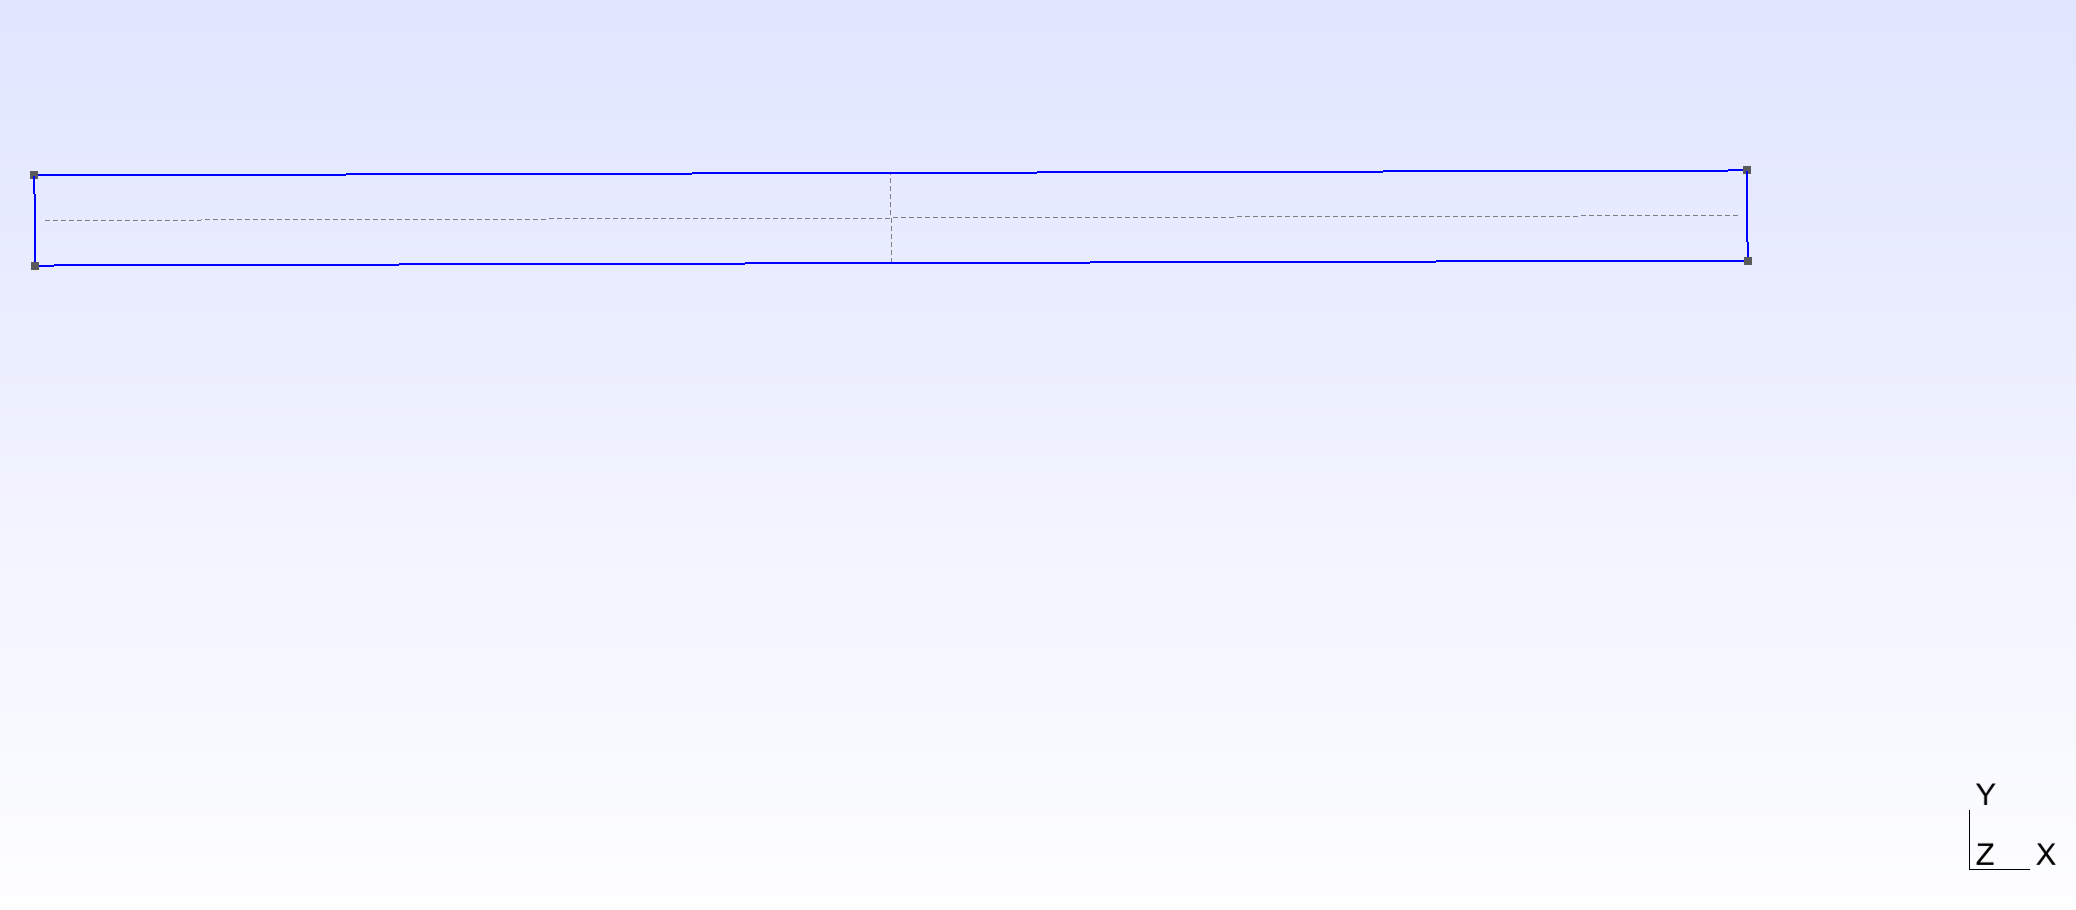
\includegraphics[height=0.26\textheight]{ch18-wag-plane.png}
\end{center}
\end{columns}
\sourcecredit{Screenshots: Julian Wag, ``Using gmsh to make 2D meshes from scratch'' (2016), gmsh 2.x on macOS.}
\end{frame}

% 14
\begin{frame}{The GUI route (2): mesh, refine, save}
\label{fr:wag2}
\scriptsize
\begin{columns}[T]
\column{0.5\textwidth}
\begin{enumerate}
  \setcounter{enumi}{3}
  \item \textbf{Modules $\to$ Mesh $\to$ 2D}. ``For some strange reason, you should click 1D and then click 2D to make it show up'' (2017); both decks say the first mesh ``might not look good, e.g.\ the tris are not even, the mesh is not refined enough.''
  \item Right- and left-click together in the canvas (or \textbf{Tools $\to$ Options $\to$ Mesh $\to$ General}): \textbf{Global mesh size factor}, type a factor (default $1$), OK; then \textbf{1D}, \textbf{2D} again to refresh.
  \item Wag's example: a rectangle $0.1\times2$ with the factor $0.1$ ``allowed even tris, with 1 on the short length and 20 on the long length'': $80$ triangles, ``four times as many triangles as tri edges in the long edge.''
  \item \textbf{File $\to$ Export} (2017: ``Save as''), \code{.msh}, Version 2 ASCII. ``Put this \code{.msh} file in the folder of your simulation and modify the \code{main.C} file to read in the mesh'': today, \code{MESH\_FILENAME = "triangle.msh"} in \code{input2d}.
\end{enumerate}
\column{0.48\textwidth}
\begin{center}
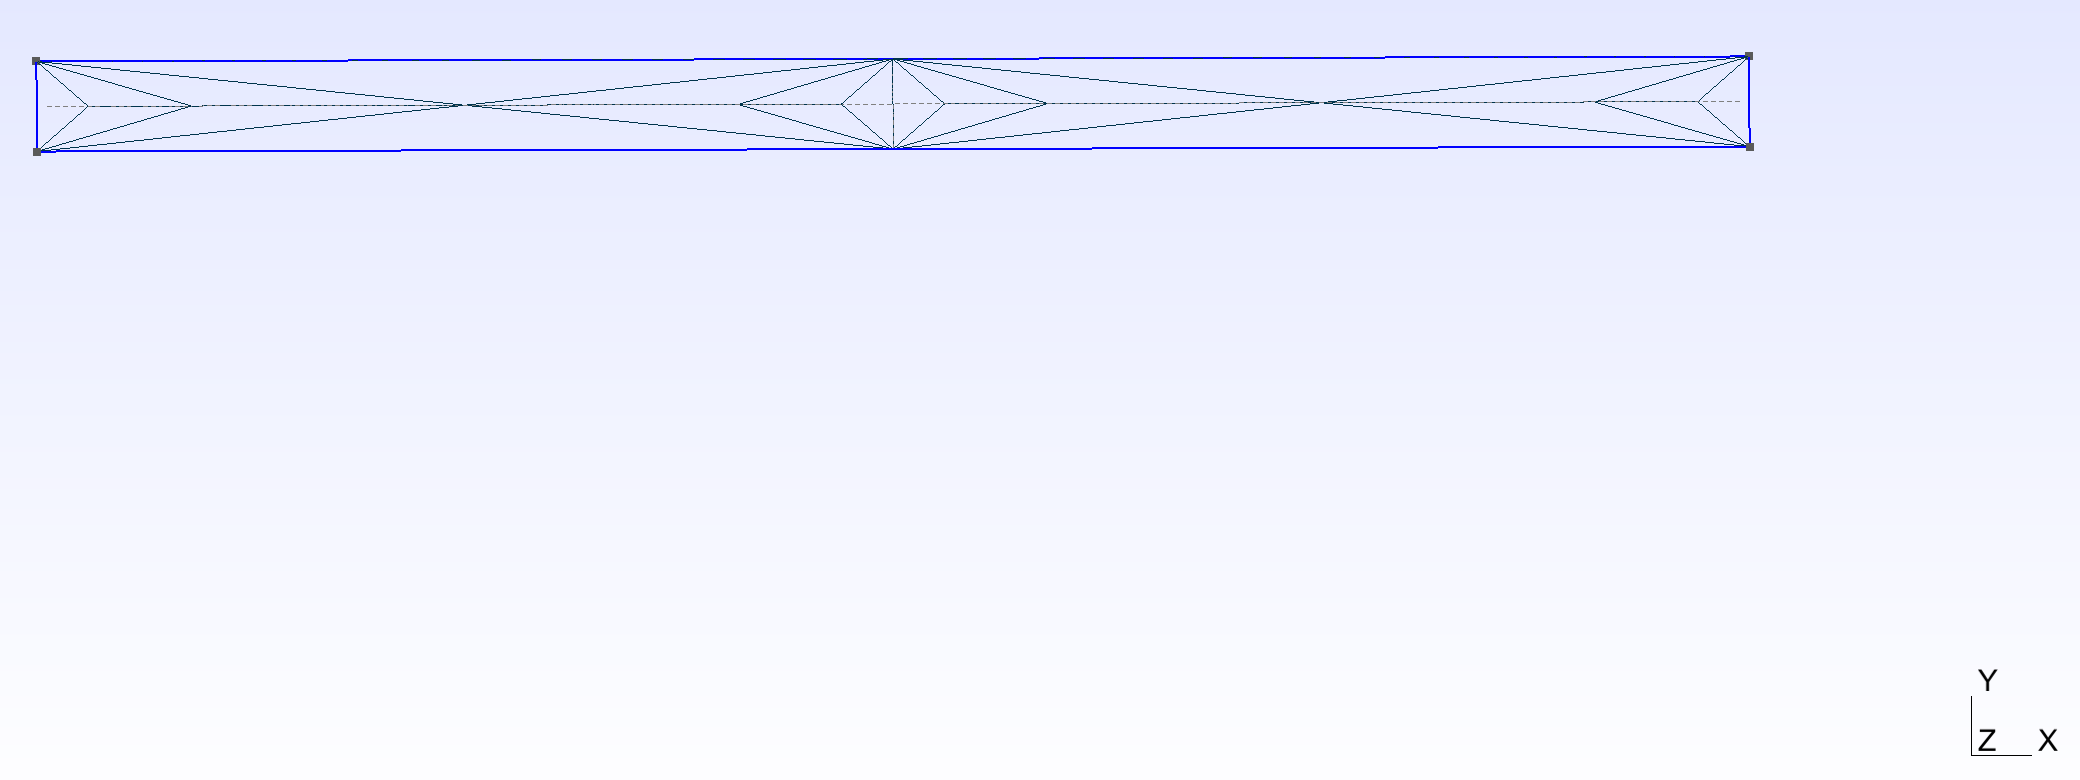
\includegraphics[height=0.20\textheight]{ch18-wag-mesh1.png}\\[2pt]
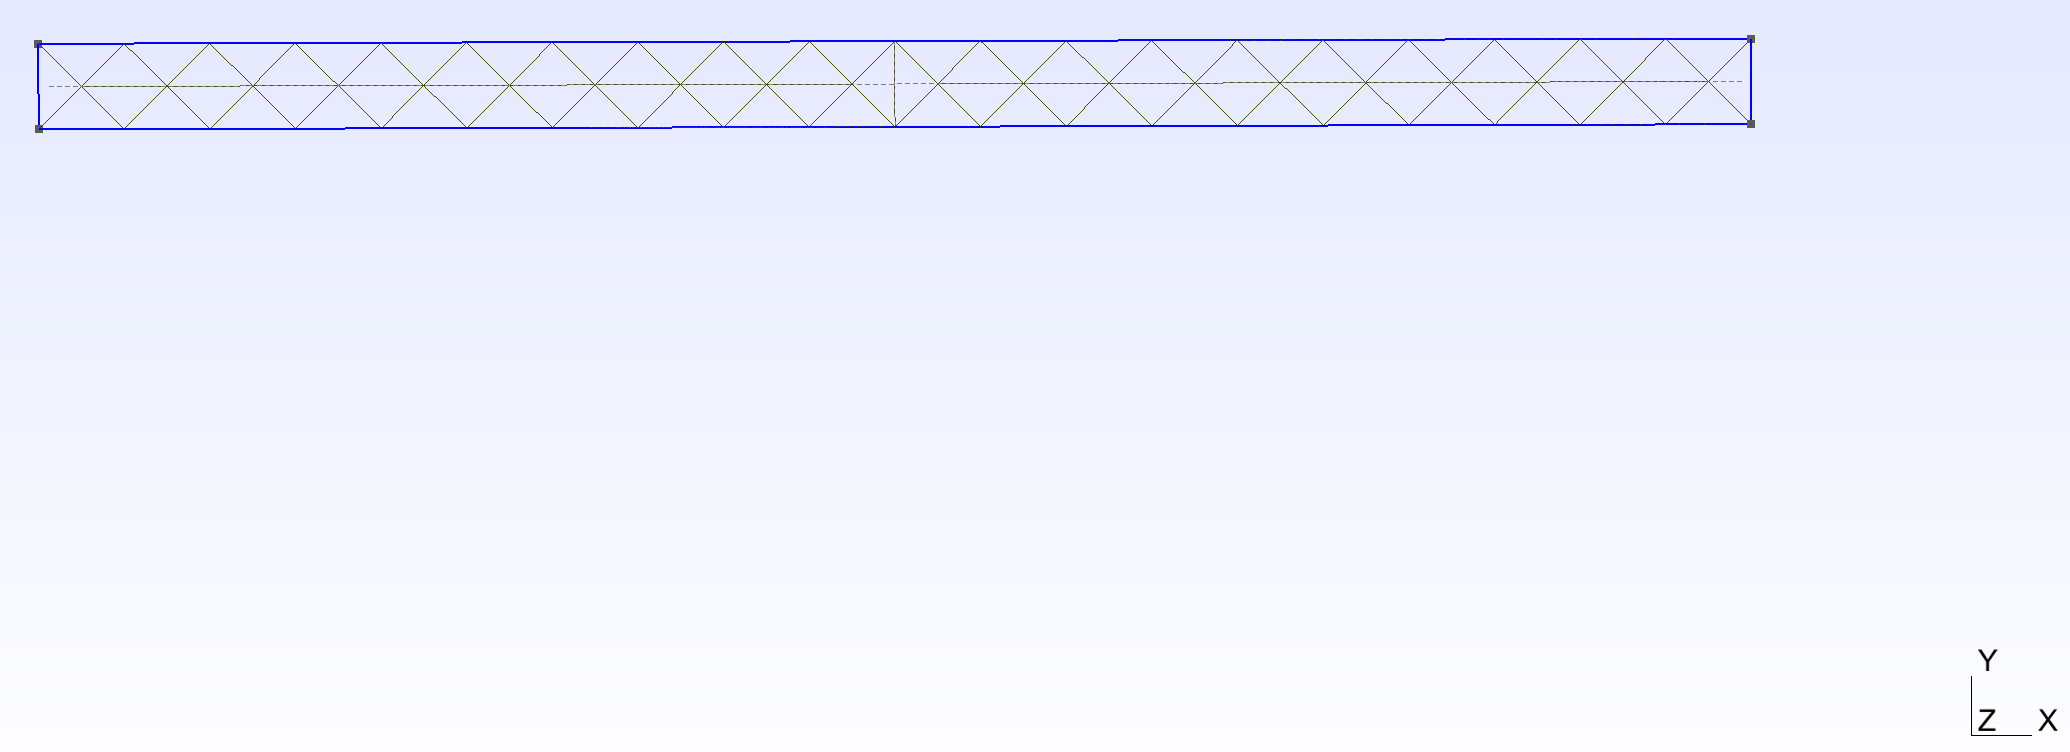
\includegraphics[height=0.20\textheight]{ch18-wag-mesh2.png}\\[2pt]
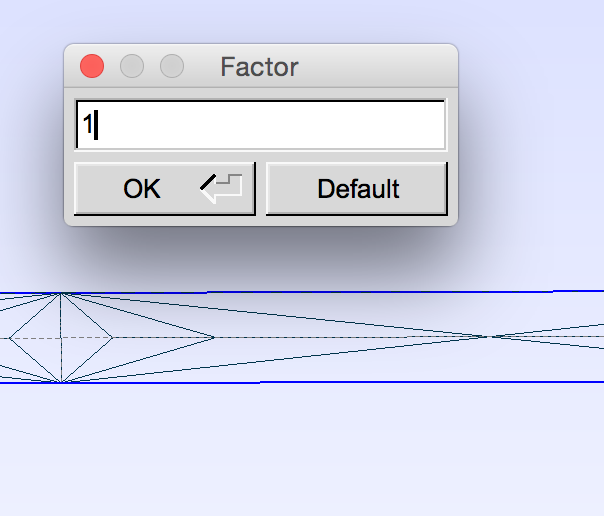
\includegraphics[height=0.15\textheight]{ch18-wag-sizefactor.png}
\end{center}
\end{columns}
\sourcecredit{Screenshots: Julian Wag (2016). Top: the first mesh; middle: after the size factor $0.1$.}
\end{frame}

% 15
\begin{frame}{The homework's last two slides: what to change in the program and the input}
\label{fr:homeworkchanges}
\footnotesize
\begin{itemize}
  \item ``In \code{main.C}, search for \code{IBFE\_Mesh2D\_128.mat}, replace with \code{triangle.msh}'' (2017--2024). In the shipped examples the name is the input key \code{MESH\_FILENAME}; nothing is recompiled.
  \item ``Changes to \code{input2d}: \code{MFAC = 1.0}, \code{IB\_POINT\_DENSITY = 1.0}. Did this to update to 1:1 ratio for boundary mesh size to Cartesian mesh size. You may also need to change \code{DT} to something smaller.'' The \code{MFAC} line does nothing to a read-in mesh (chapter 17); the point density does, and IBFE/05 keeps $1.0$ because its elements are one grid cell across (slide \ref{fr:rules}). Its \code{DT} is $5\times10^{-4}$, half of IBFE/01's: the smaller elements and the sharper corners of the triangle move faster fluid near them.
  \item ``Run simulation: here is mine with both grids!'' (the slide showed the triangle on the AMR patches). IBFE/05's README has the numbers: the centre rises from $y = 0.168$ to $0.668$ at $t = 1$ (the top corner reaches $0.997$, just under the top of the box), returns, is released at $t = 3$ and sinks to $-0.740$ by $t = 4$, turning as it goes; every node stays within $0.011$ of its target while tethered.
  \item The 2017 copy of the homework was a zip, \code{Example\_IBFE\_TetherForceFullTriangle2D\_2016-11.zip}, with \code{Beam\_IBFE\_Mesh2D.m} and the \code{.mat} plate still inside, unused: the same mismatch as chapter 17's extras.
\end{itemize}
\begin{punchbox}
\footnotesize A new mesh is a new structure: check that it fits the box, re-choose the point density and the time step, and expect different numbers. The homework's own warning was ``you may also need to change \code{DT}.''
\end{punchbox}
\end{frame}

% 16
\begin{frame}[fragile]{Battista's tube tutorial (1): parameters, poles, arcs}
\label{fr:battista}
\footnotesize
\emph{How To Make Simple Geometries in Gmsh} (Nick Battista, 24 September 2014) builds a tube by mouse and text together. Its steps, with the \code{.geo} lines they produce:
\begin{enumerate}
  \item \textbf{File $\to$ Save As} \code{geometry.geo} first (``the first obstacle: getting the file to save where you want it''), then \textbf{Modules $\to$ Geometry $\to$ Reload}.
  \item \textbf{Elementary entities $\to$ Parameters}: $L = 2.0$ (length), $r = 0.25$ (radius). Then \textbf{Edit file} (``once you get the hang of gmsh, this will be your best friend''; Windows users: set the editor command to \code{C:/Windows/notepad.exe \%s}) and add an element size:
\begin{lstlisting}[style=geotiny]
ds = DefineNumber[ L/100.0, Name "Parameters/r" ];   // the tutorial's line; the Name should be "Parameters/ds"
\end{lstlisting}
  The name is the label in the GUI's parameter list; reusing \code{"Parameters/r"} ties \code{ds} to the slider called $r$, so the tutorial's own figure shows two parameters named $r$. Write \code{"Parameters/ds"}.
  \item \textbf{Point}: five points for the first circle, the centre and the four ``poles'' (N, S, E, W) at $z = +L/2$, each with \code{ds} as the prescribed mesh element size (``add \code{ds} to prescribed mesh element size at point''); the other four typed into the file.
  \item \textbf{Circle arc}: three clicks per arc, ``the point where the arc starts, the central point, the point where the arc ends'' (an arc is less than a half turn, so a circle needs four); ``I am doing everything going counter-clockwise. It's good just to keep a constant convention.''
  \item The second circle at $z = -L/2$ ``completely in the text-file''; then four straight lines between matching poles: \code{Line(11) = \{3, 8\}; Line(12) = \{4, 9\};} and the note on shared numbering (slide \ref{fr:gmshbasics}).
\end{enumerate}
\end{frame}

% 17
\begin{frame}[fragile]{Battista's tube tutorial (2): surfaces, and where it stops}
\label{fr:battista2}
\footnotesize
\begin{enumerate}
  \setcounter{enumi}{5}
  \item \textbf{Ruled Surface} (gmsh 4: \textbf{Surface}): click \code{Circle(1)}, \code{Line(9)}, \code{Circle(5)}, \code{Line(10)}, press \textbf{e}: one quarter of the curved wall; the other three the same way or in the file. ``Note the dotted lines signifying a surface.''
  \item \textbf{Mesh $\to$ 2D}: the wall is meshed with triangles.
  \item For a closed tube, \textbf{Plane Surface} on the four arcs of each end; \textbf{e}.
\end{enumerate}
The tutorial ends there, with a surface mesh and no file saved. What IBFE needs is a \emph{volume} mesh in a file:
\begin{lstlisting}[style=geotiny]
Surface Loop(100) = {14, 16, 18, 20, 21, 22};   // the four wall pieces and the two caps
Volume(101) = {100};
Physical Volume("tube") = {101};                 // so that only the tetrahedra are saved
// then:  gmsh -3 -format msh22 geometry.geo -o tube.msh
\end{lstlisting}
\begin{itemize}
  \item A hollow tube (a vessel wall) is two concentric circles per end and the same construction twice; the course's \code{tube.geo} (slide \ref{fr:samples}) does it with transfinite hexahedra instead, and chapter 24's tube example uses a 2D section.
  \item The crosswalk's other notes on this document: \code{Ruled Surface} and \code{Line Loop} are gmsh-2 names (accepted by gmsh 4.12 with no warning in the runs of slide \ref{fr:run}); the ONELAB parameter name is duplicated (above); the tutorial is Battista's and is cited, not copied.
\end{itemize}
\end{frame}

% 18
\begin{frame}[fragile]{The course's four sample \code{.geo} files, run today}
\label{fr:samples}
\scriptsize
\begin{tabular}{@{}L{0.12\textwidth}L{0.36\textwidth}L{0.44\textwidth}@{}}
\toprule
file & what it does & \code{gmsh -3 -format msh22}, gmsh 4.12.1 \\
\midrule
\code{cube.geo} & a unit square (\code{lc = 0.3}) extruded by $(0, 0, 1)$ into a volume; \code{Physical Volume(1) = tmp[1];} takes the volume the extrusion returned & $141$ nodes, $373$ \code{TET4}; nothing else saved, because of the physical volume \\
\code{cone.geo} & a triangle in the $xz$-plane revolved four times by $\pi/2$ about the $z$ axis (\code{Extrude \{\{0,0,1\}, \{0,0,0\}, Pi/2\} \{ Surface\{5\}; \}} four times, each on the surface the last one produced); no physical group & $648$ nodes, $3845$ elements: $2460$ \code{TET4}, $1248$ \code{TRI3}, $131$ lines, $6$ points. libMesh reads the tetrahedra as the mesh and files the rest as boundary information; add \code{Physical Volume} to keep the file small \\
\code{sphere.geo} & eight circle arcs on three great circles, eight \code{Ruled Surface}s, a surface loop, a volume; \code{Physical Surface} and \code{Physical Volume}; \code{Mesh.Algorithm = 6}; \code{lc = .55} & $60$ nodes, $114$ \code{TET4} and $114$ \code{TRI3} (the surface group): far too coarse for a body in a flow, a demonstration of the construction \\
\code{tube.geo} & a tube of length $10$ and diameter $1$ built from $34$ points and $73$ curves, \code{Transfinite} everything, \code{Recombine Surface "*"}, \code{Transfinite Volume "*"}, physical groups \code{inlet}, \code{outlet}, \code{walls}, \code{tube}; ends with \code{Mesh 3; Save "tube.msh";} & $593{,}800$ nodes, $579{,}488$ \code{HEX8} and $28{,}112$ \code{QUAD4}; $80$ MB. The densities \code{den1 = 15}, \code{den2 = 20}, \code{den3 = 200} are the counts across, radially and along; $6/5/24$ give the picture's $2{,}784$ hexahedra \\
\bottomrule
\end{tabular}

\end{frame}

% 19
\begin{frame}{The four samples, meshed}
\label{fr:samplepics}
\begin{columns}[T]
\column{0.25\textwidth}\centering 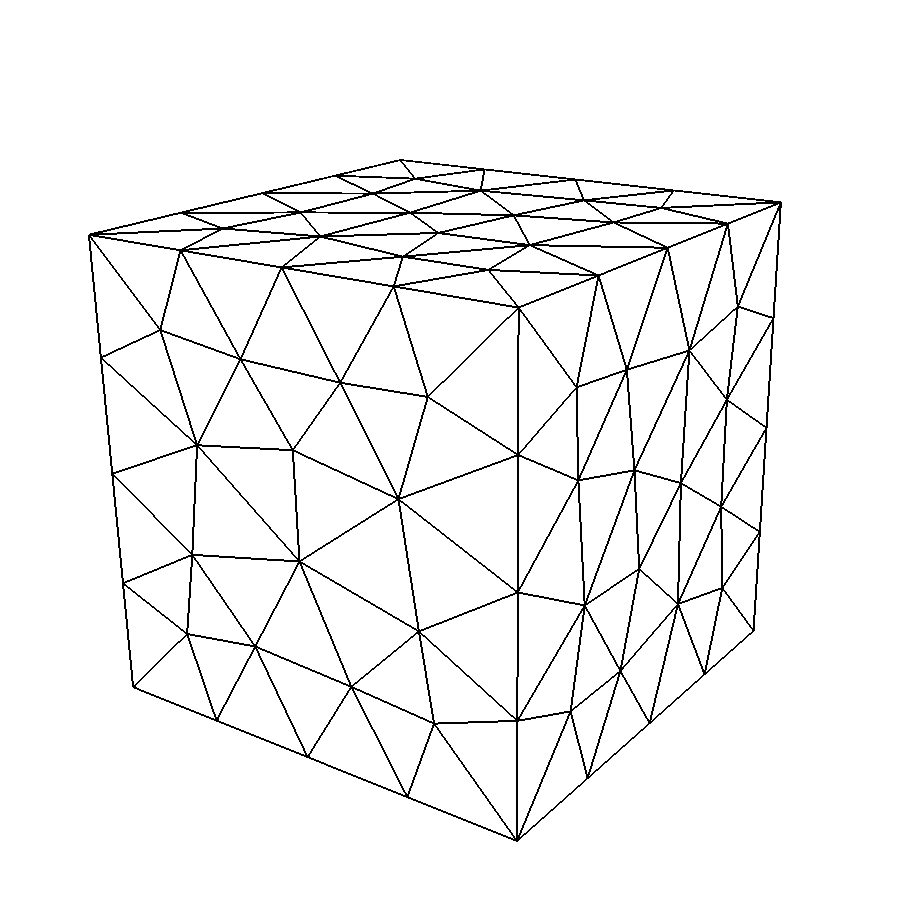
\includegraphics[width=\textwidth]{ch18-cube-gmsh.png}\\ \scriptsize \code{cube.geo}: extrusion, $373$ tets
\column{0.25\textwidth}\centering 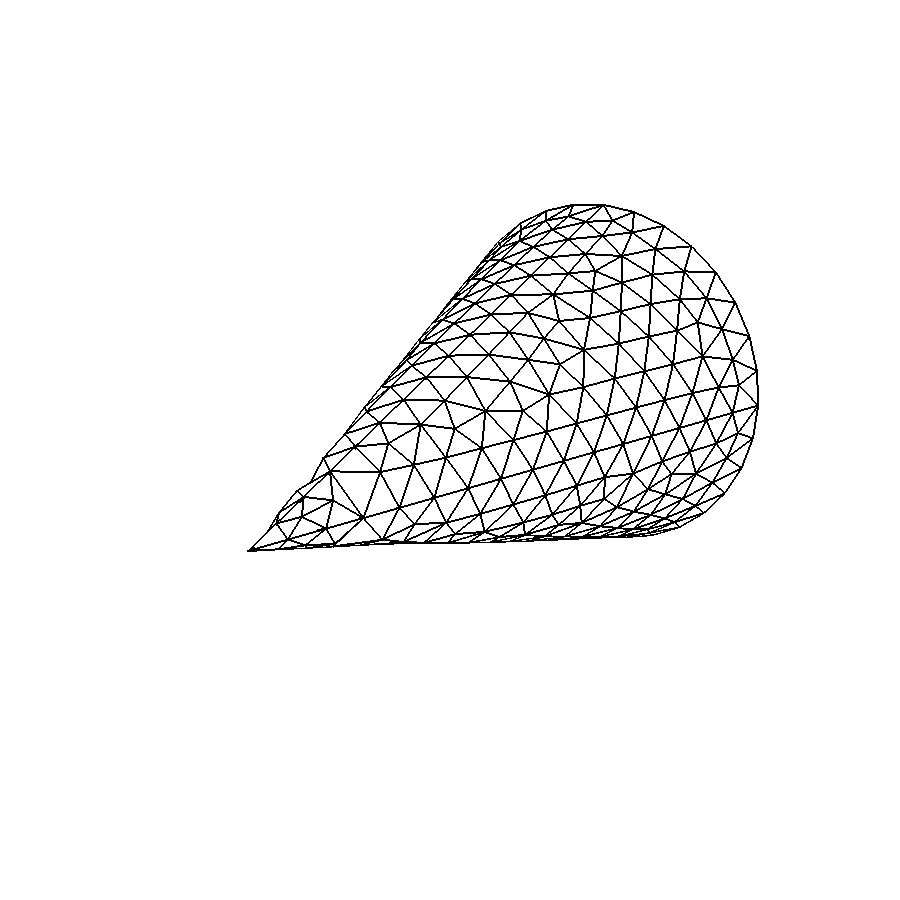
\includegraphics[width=\textwidth]{ch18-cone-gmsh.png}\\ \scriptsize \code{cone.geo}: four revolutions, $2460$ tets
\column{0.25\textwidth}\centering 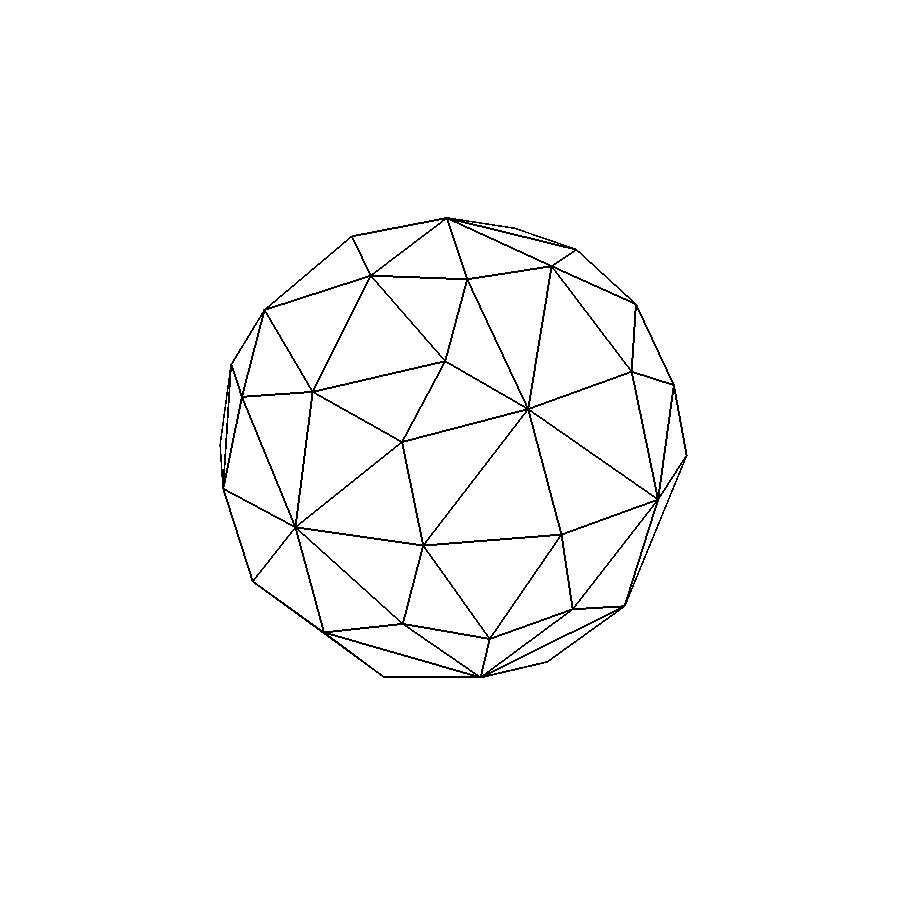
\includegraphics[width=\textwidth]{ch18-sphere-gmsh.png}\\ \scriptsize \code{sphere.geo}: $114$ tets at \code{lc = 0.55}
\column{0.25\textwidth}\centering 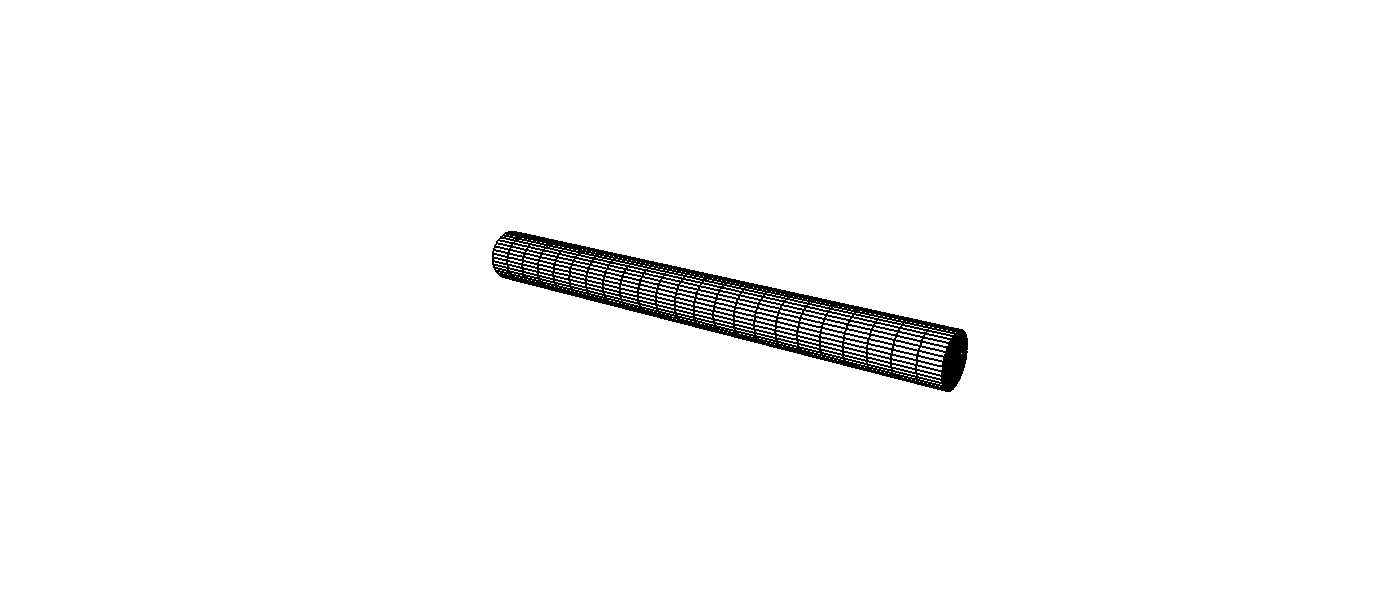
\includegraphics[width=\textwidth]{ch18-tube-gmsh.png}\\ \scriptsize \code{tube.geo} at $6/5/24$: $2784$ hexes
\end{columns}
\scriptsize
\begin{itemize}
  \item Rendered in VisIt from VTK copies (\code{gmsh x.msh -save -format vtk -o x.vtk}); VisIt does not read \code{.msh} itself. Chapter 27 does the same with the 3D results.
  \item The tube is the only hexahedral mesh in the course material; everything from gmsh's free meshers is tetrahedra. Hexahedra need a structured construction (transfinite blocks, as here) or Coreform Cubit (slide \ref{fr:cubit}).
  \item These four files sit next to Battista's PDF in every copy of the meshing folder, with no read-me of their own; they are the ``examples'' the Trelis read-me and the meshing read-me refer to. No warnings and no errors from gmsh 4.12.1 for any of them.
\end{itemize}
\sourcecredit{\code{wsl/final/ch18\_meshtest.sh} and \code{ch18\_render.sh}; gmsh 4.12.1, VisIt 3.5.}
\end{frame}

% 20
\begin{frame}[fragile]{A 3D gmsh mesh IBFE actually runs: the plate of IBFE/10}
\label{fr:plate2}
\scriptsize
\begin{columns}[T]
\column{0.5\textwidth}
\begin{lstlisting}[style=datatiny]
$MeshFormat
2.2 0 8
$EndMeshFormat
$PhysicalNames
1
3 1 "plate2"
$EndPhysicalNames
$Nodes
3386
1 0 1 1
2 0 -1 1
3 0 -1 -1
...
\end{lstlisting}
\begin{itemize}
  \item \code{plate2.msh} (2017): a plate $0.125$ thick and $2\times2$, $3{,}386$ nodes, $11{,}481$ \code{TET4}, one physical volume named \code{plate2}; element size about three fine cells ($\Delta x = 1/16$ in the tank). Its \code{.geo} is lost; the 2020 flow-tank deck (chapter 22) shows the GUI steps that made it.
  \item The physical name becomes the libMesh subdomain name (\code{mesh.subdomain\_name(id) = phys\_name}, \code{gmsh\_io.C}); \code{mesh.get\_id\_by\_name("plate2")} returns the id.
\end{itemize}
\column{0.48\textwidth}
\begin{center}
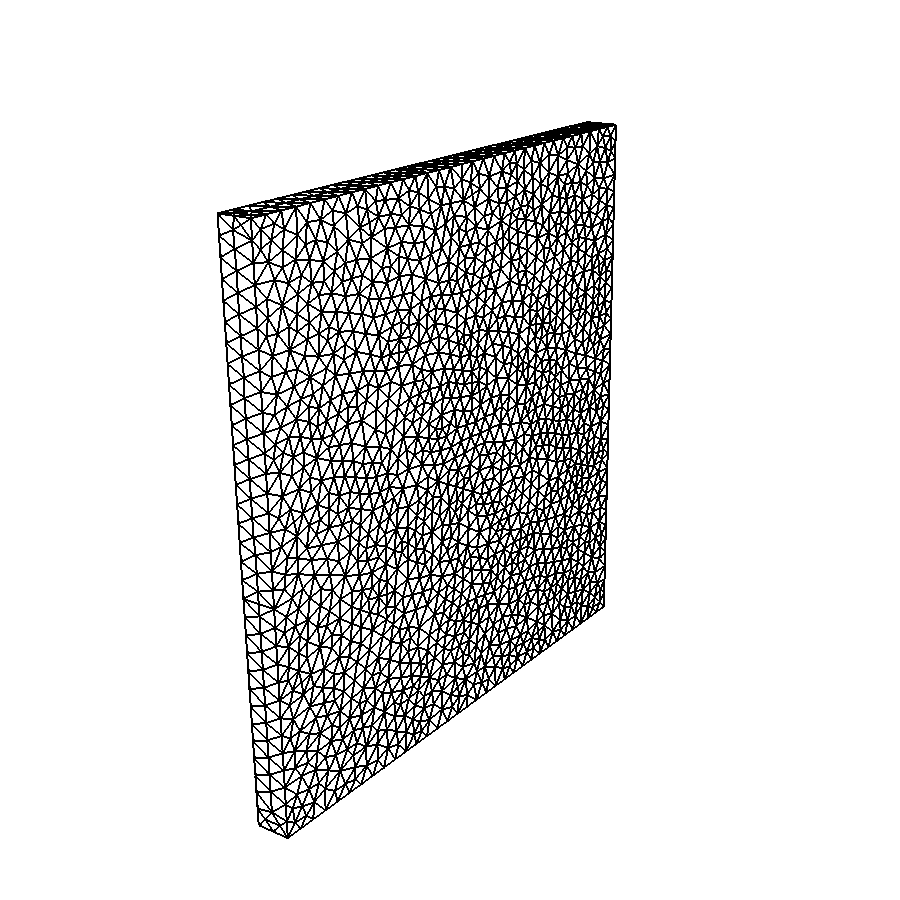
\includegraphics[width=0.78\textwidth]{ch18-plate2-gmsh.png}
\end{center}
\end{columns}
\end{frame}

% 21
\begin{frame}{gmsh physical groups and what libMesh makes of them}
\label{fr:physical}
\scriptsize
\begin{tabular}{@{}L{0.30\textwidth}L{0.62\textwidth}@{}}
\toprule
in the \code{.geo} & in libMesh after \code{mesh.read()} (\code{gmsh\_io.C}, libMesh 1.7.8) \\
\midrule
\code{Physical Surface("triangle", 1)} in a 2D mesh, \code{Physical Volume("plate2")} in 3D & the elements get \code{subdomain\_id = 1}; \code{mesh.subdomain\_name(1) = "triangle"}. Several groups: several subdomains, which chapter 21 uses to give parts of one mesh different stresses (\code{elem->subdomain\_id()} inside a stress function). \\
\code{Physical Curve} in 2D, \code{Physical Surface} in 3D (a group one dimension below the mesh) & the elements are not kept as elements; each becomes a side set entry on the element it borders, named after the group (\code{sideset\_name}); nodes of a \code{Physical Point} become a node set. These are the boundary ids a program can test with \code{boundary\_info.has\_boundary\_id(elem, side, id)}. \\
a lower-dimensional group whose name contains \code{lower\_dimensional\_block} & kept as elements of a lower dimension (libMesh's escape hatch for fractures and shells); not for IBFE. \\
no physical group at all & every element of every dimension is saved and read; the highest dimension is the mesh, the rest become boundary information. Works, but \code{cone.msh} was three times its necessary size. \\
\bottomrule
\end{tabular}

\begin{punchbox}
\footnotesize One rule covers it: give the body a \code{Physical Surface} (2D) or \code{Physical Volume} (3D), and give any boundary you want to name a physical group one dimension lower. The IBFE examples here need only the first.
\end{punchbox}
\end{frame}

% 22
\begin{frame}[fragile]{Route C: the \code{.poly} file}
\label{fr:poly}
\scriptsize
Triangle (Jonathan Shewchuk, 2D) and TetGen (Hang Si, 3D) mesh a \emph{piecewise linear complex} written in a \code{.poly} file: ``The \code{.poly} alone is not the mesh but rather a file that you input to the mesh generator'' (2014). Its four parts:
\begin{tabular}{@{}L{0.14\textwidth}L{0.40\textwidth}L{0.38\textwidth}@{}}
\toprule
part & 2D (Triangle) & 3D (TetGen) \\
\midrule
1. nodes & \code{<\# points> <2> <\# attributes> <marker 0/1>}, then \code{<\#> <x> <y> [attr] [marker]} & \code{<\# points> <3> <\# attributes> <marker 0/1>}, then \code{<\#> <x> <y> <z> [attr] [marker]} \\
2. segments / facets & \code{<\# segments> <marker 0/1>}, then \code{<\#> <node> <node> [marker]} & \code{<\# facets> <marker 0/1>}, then for each facet \code{<\# polygons> [<\# holes>] [marker]}, each polygon \code{<\# corners> <node> ...}, then the facet's hole points \\
3. holes & \code{<\# holes>}, then \code{<\#> <x> <y>}: one point inside each cavity & \code{<\# holes>}, then \code{<\#> <x> <y> <z>} \\
4. regions (optional) & \code{<\# regions>}, then \code{<\#> <x> <y> <attribute> <max area>} & \code{<\# regions>}, then \code{<\#> <x> <y> <z> <attribute> <max volume>} \\
\bottomrule
\end{tabular}

\medskip
\begin{itemize}
  \item ``The first three parts are mandatory, but the fourth part is optional'' (2014); a file with no holes still needs the line \code{0}.
  \item Node numbers start at $1$ (or $0$: the meshers follow the first node's number; libMesh's reader handles both).
  \item A marker on a segment or facet is a boundary id; a region attribute becomes a subdomain id (libMesh's \code{TetGenIO} reads it as the element's \code{subdomain\_id} when the \code{.ele} file carries attributes).
\end{itemize}
\end{frame}

% 23
\begin{frame}[fragile]{Triangle on the course's \code{.poly}}
\label{fr:triangle}
\footnotesize
\begin{columns}[T]
\column{0.5\textwidth}
\code{IBFE\_Mesh2D\_128.poly}, written by \code{Beam\_IBFE\_Mesh2D.m} (chapter 17, slide 40): a $1.0 \times 0.25$ rectangle with $84$ nodes along its outline, no holes:
\begin{lstlisting}[style=datatiny]
84 2 0 1
1 -5.0000000000000000e-01 1.2500000000000000e-01 1
2 -4.7500000000000000e-01 1.2500000000000000e-01 1
...
84 2 0 1
1 1 2 1
...
0
\end{lstlisting}
\begin{lstlisting}[style=shell]
triangle -pq IBFE_Mesh2D_128.poly
# -p: read a .poly; -q: quality mesh (no angle below 20 degrees)
# -a0.001 would limit the triangle area; -o2 makes 6-node triangles
\end{lstlisting}
Output: \code{IBFE\_Mesh2D\_128.1.node} ($122$ nodes), \code{.1.ele} ($162$ triangles), \code{.1.poly}. The \code{.1} is Triangle's iteration number.
\column{0.48\textwidth}
\begin{center}
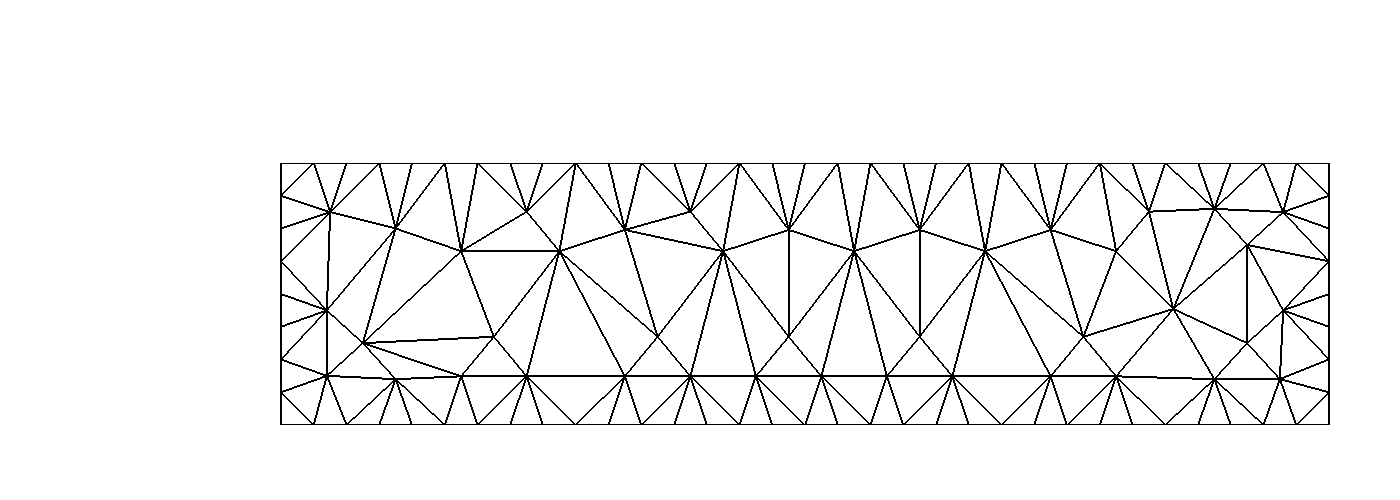
\includegraphics[width=\textwidth]{ch18-plate-triangle.png}
\end{center}
\scriptsize The $162$ triangles Triangle makes with \code{-pq} and no area limit: one row across the width, since the outline's spacing ($0.025$) sets the size at the edges and nothing refines the interior.
\begin{itemize}
  \item libMesh's \code{TetGenIO} is three-dimensional (it sets \code{mesh\_dimension(3)}), so a Triangle result does not go straight into \code{main2d}. Convert it (slide \ref{fr:readtetgen}) or make the 2D mesh with gmsh.
  \item libMesh can also call Triangle and TetGen itself (\code{TriangleInterface}, \code{TetGenMeshInterface}) when it was built with them; autoibamr's libMesh is built without, so the command line is the way.
\end{itemize}
\end{columns}
\end{frame}

% 24
\begin{frame}[fragile]{TetGen on a unit cube, and the ``Generating your elements'' slide that was never written}
\label{fr:tetgenrun}
\scriptsize
\begin{columns}[T]
\column{0.5\textwidth}
\code{cube.poly}: eight corners, six square facets, no holes, no regions:
\begin{lstlisting}[style=datatiny,aboveskip=2pt,belowskip=0pt]
# a unit cube: 8 nodes, 6 facets, no holes
8 3 0 0
1 0 0 0
2 1 0 0
3 1 1 0
4 0 1 0
5 0 0 1
6 1 0 1
7 1 1 1
8 0 1 1
6 0
1
4 1 2 3 4
1
4 5 6 7 8
1
4 1 2 6 5
1
4 2 3 7 6
1
4 3 4 8 7
1
4 4 1 5 8
0
0
\end{lstlisting}
\column{0.48\textwidth}
\begin{lstlisting}[style=shell]
tetgen -pq1.4a0.02 cube.poly
# -p: read a .poly; -q1.4: quality (radius-edge ratio <= 1.4)
# -a0.02: no tetrahedron larger than 0.02; -k: also write a .vtk
\end{lstlisting}
Output: \code{cube.1.node} ($75$ nodes), \code{cube.1.ele} ($153$ tetrahedra), \code{cube.1.face}, \code{cube.1.edge}.
\end{columns}
\end{frame}

% 24b
\begin{frame}{TetGen on a unit cube (2): the result, and how a facet is written}
\label{fr:tetgenrun2}
\begin{columns}[T]
\column{0.42\textwidth}
\begin{center}
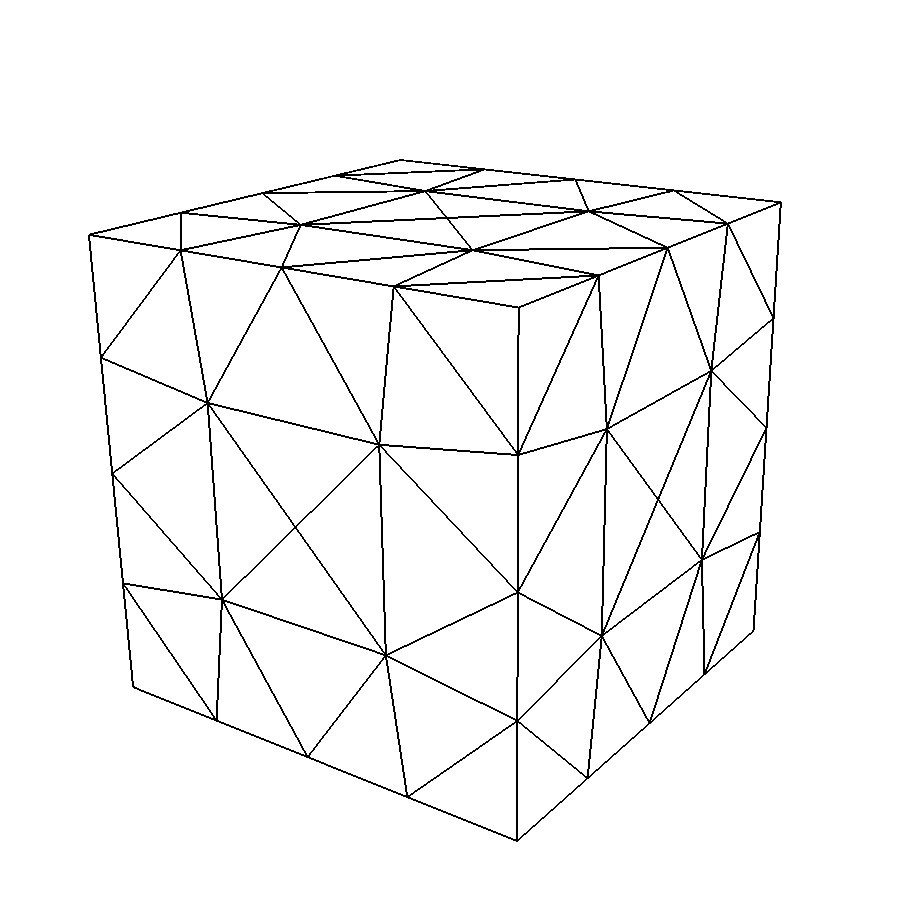
\includegraphics[width=0.9\textwidth]{ch18-cube-tetgen.png}
\end{center}
\column{0.56\textwidth}
\footnotesize Each facet line is \code{<\# polygons> [holes] [marker]} then \code{<\# corners> <nodes>}; a facet with a hole lists two polygons (the outer and the inner boundary) and then the hole point inside the facet. The \code{-a} value is what sets the element size; without it TetGen only fills the hull with the fewest tetrahedra it can.
\end{columns}
\end{frame}

% 25
\begin{frame}[fragile]{Holes and regions: the other slide that was never written}
\label{fr:holes}
\footnotesize
\begin{columns}[T]
\column{0.5\textwidth}
A 2D plate with a round hole, for Triangle (\code{plate\_hole.poly}): the outline, a $12$-gon inside it, and one hole point:
\begin{lstlisting}[style=datatiny]
16 2 0 1          # 4 corners + 12 points on the hole
1 -0.5 -0.125 1
2  0.5 -0.125 1
3  0.5  0.125 1
4 -0.5  0.125 1
5  0.06 0.0 2     # the 12 hole points, radius 0.06, marker 2
...
16 1              # 16 segments: 4 outer + 12 inner
1 1 2 1
...
1                 # one hole
1 0.0 0.0         # any point inside the hole
\end{lstlisting}
\begin{lstlisting}[style=shell]
triangle -pqa0.0005 plate_hole.poly
\end{lstlisting}
Triangle removes every triangle it can reach from the hole point without crossing a segment: that is what ``a list of hole points'' means.
\column{0.48\textwidth}
\begin{itemize}
  \item In 3D the same: a cavity is a closed set of facets and one point inside it, listed in part 3. A \emph{facet} hole (a window in a flat face) is listed inside the facet, after its polygons.
  \item \al{Regions} (part 4) do the opposite of holes: a point inside a closed region gives all elements there an attribute (a subdomain id for libMesh) and a size limit. Two regions in one file: a stiff core and a soft rind, or a stem and a leaf (chapter 22's two-stiffness plate does this with a position test instead).
  \item IBFE does not need holes for fluid passages: the fluid is everywhere already, and a hole in the solid is simply fluid. Use a hole for a geometric hole in the body.
  \item The 2014 slides ``Holes'' and ``Generating your elements'' were headings with nothing under them; this slide and the last are what they would have said.
\end{itemize}
\end{columns}
\end{frame}

% 26
\begin{frame}[fragile]{Reading TetGen (and Triangle) output}
\label{fr:readtetgen}
\footnotesize
\scriptsize The 2014 code, which still compiles once \code{Mesh mesh(NDIM)} becomes the communicator form:
\begin{lstlisting}[style=cpptiny]
#include <libmesh/tetgen_io.h>
...
Mesh mesh(init.comm(), NDIM);
TetGenIO TETGEN(mesh);
// the course wrote "Jellyfish_IBFE_Mesh3D.ele";
// that file is in no archive
TETGEN.read("example_IBFE_Mesh3D.ele");
mesh.prepare_for_use();
\end{lstlisting}
\begin{itemize}
  \item \code{TetGenIO::read(name)} takes either name of the pair and derives the other (\code{tetgen\_io.C}: ``Check name for \code{*.node} or \code{*.ele} extension''); both files must be there, or \code{Error while opening either ... or ...}. \code{mesh.read("cube.1.ele")} does the same through \code{NameBasedIO}, so the explicit \code{TetGenIO} is optional.
  \item It is 3D only (``tetgen only works in 3D''): Triangle's 2D \code{.node}/\code{.ele} pair must become something else for \code{main2d}. Twenty lines of Python turn it into MSH 2.2 (the format of slide \ref{fr:plate2}: a \code{\$Nodes} block with \code{<\#> <x> <y> 0}, an \code{\$Elements} block with \code{<\#> 2 2 1 1 <n1> <n2> <n3>}), or into legacy VTK for a look in VisIt (\code{wsl/final/ch18\_render.sh} does the latter for the plate above). Or skip Triangle: gmsh meshes the same outline from a \code{.geo} with the hole as a second curve loop.
  \item A TetGen \code{.ele} file with region attributes (\code{tetgen -pA}) gives each tetrahedron a \code{subdomain\_id}; without \code{-A} every element is subdomain $0$.
  \item Node and element numbering start at $1$ in TetGen's output unless the input started at $0$; libMesh's reader renumbers either way.
\end{itemize}
\end{frame}

% 27
\begin{frame}{Route D: from a CAD model to a mesh}
\label{fr:cad}
\footnotesize
\begin{tabular}{@{}L{0.22\textwidth}L{0.70\textwidth}@{}}
\toprule
stage & tools and notes \\
\midrule
make the solid & Fusion 360 (the two corals of chapter 21), SolidWorks, Blender (the hollow carotid of the coming example), SpaceClaim; or a scan (micro-CT, laser) that gives a surface \\
export & STEP or IGES for a true solid; STL for a triangulated surface (what scans and Blender give). The 2020 tool list also had Meshmixer for cleaning STL surfaces; Autodesk discontinued it in 2021, and Blender's remesh tools or MeshLab do the job now. \\
mesh the solid & \al{Coreform Cubit} (formerly Trelis, before that Bolt and Cubit from csimsoft/Sandia): imports STEP and STL, makes tetrahedra or, with the pave-and-sweep workflow, hexahedra; exports ExodusII (\code{.e}) with named blocks and side sets. \al{gmsh}: imports STEP (\code{Merge "part.step";}) and STL (\code{Merge "part.stl";} then \code{Surface Loop}, \code{Volume} on the classified surface); tetrahedra only. \\
read & \code{mesh.read("part.e")}: Exodus blocks become subdomains (next slide); \code{mesh.read("part.msh")} as above. \\
check & slide \ref{fr:checks}: dimension, size, orientation, position, element count. \\
\bottomrule
\end{tabular}

\end{frame}

% 27b
\begin{frame}{Route D (2): Trelis, Bolt, Coreform Cubit, and what is only listed}
\label{fr:cad2}
\footnotesize
\begin{itemize}
  \item The 2016 Trelis read-me: ``Boyce, Jeremy and I have a single floating license to Trelis''; ``Bolt, an improved Trelis'' (the licence was later confirmed, per the 2017 Read Me: ``We now have a license for Bolt''). Coreform bought Trelis in 2020 and sells it as Cubit; the csimsoft tutorial links in the read-mes are dead, \url{https://coreform.com} has their successors. The vendor's \emph{Getting Started with Trelis} PDF (2014, a brick with a hole, 116 screenshots) is third-party material and is only linked.
  \item The only Coreform Cubit material of Laura's own is a July 2022 recording (listed, chapter 0.1); chapter 21 reproduces the Fusion 360 $\to$ Bolt hex-mesh route of the two-coral example from its 2018 slides.
\end{itemize}
\end{frame}

% 28
\begin{frame}{Route D (3): the 2016 Trelis notes, and ExodusII in libMesh}
\label{fr:cubit}
\scriptsize
\begin{columns}[T]
\column{0.5\textwidth}
From the lab's 2016 ``Trellis Notes'' (private Drive; reported by the crosswalk, not reproduced in full):
\begin{itemize}
  \item hex-mesh a body by \emph{paving} one face with quadrilaterals and \emph{sweeping} it through the volume;
  \item \emph{merge} coincident surfaces of adjacent volumes so the mesh is conforming;
  \item keep walls at least $4\,\Delta x$ thick, so that there are elements across the thickness and the fluid cannot see through;
  \item FE size : Navier--Stokes grid size $= 1{:}1$.
\end{itemize}
The first two are Cubit workflow, still current; the last two are element-size rules, reconciled on slide \ref{fr:rules}.
\column{0.48\textwidth}
What libMesh does with an Exodus file (\code{exodusII\_io.C}):
\begin{itemize}
  \item each \emph{element block} becomes a subdomain: \code{subdomain\_id = block id}, \code{subdomain\_name = block name}; the block's element type sets the libMesh type (\code{TRI3}, \code{HEX8}, ...);
  \item \emph{side sets} and \emph{node sets} become boundary ids and names;
  \item nodal and elemental variables stored in the file can be read into systems (\code{ExodusII\_IO::copy\_nodal\_solution}), which is how a mesh can carry a fibre direction (chapter 20).
\end{itemize}
IBFE/08's \code{beam.e} ($98$ nodes, $126$ \code{TRI3}) and \code{circle.e} ($977$ nodes, $1851$ \code{TRI3}) came from Trelis: one block each, no sets, two-dimensional.
\end{columns}
\begin{center}
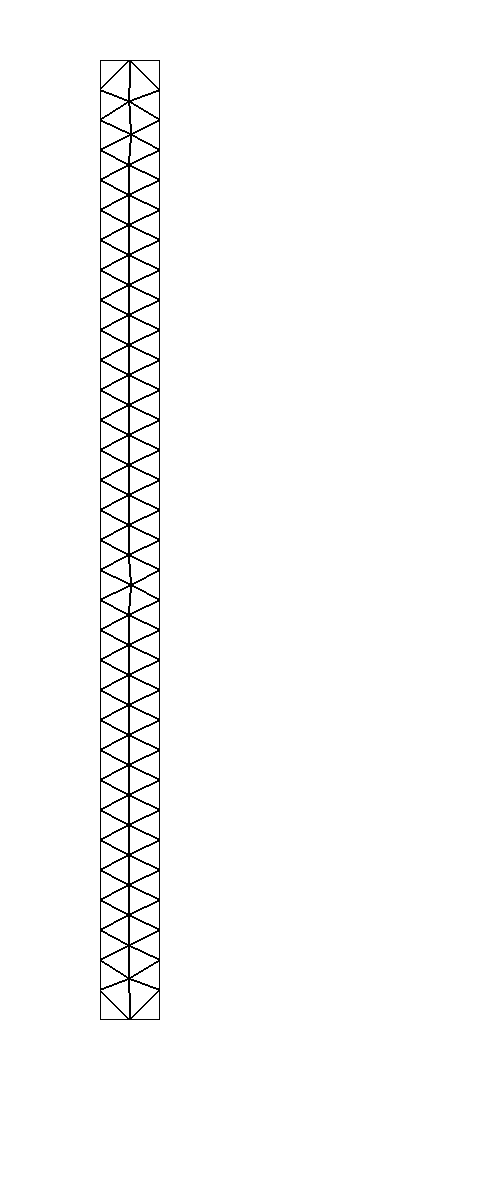
\includegraphics[height=0.13\textheight]{ch18-beam-trelis.png}\quad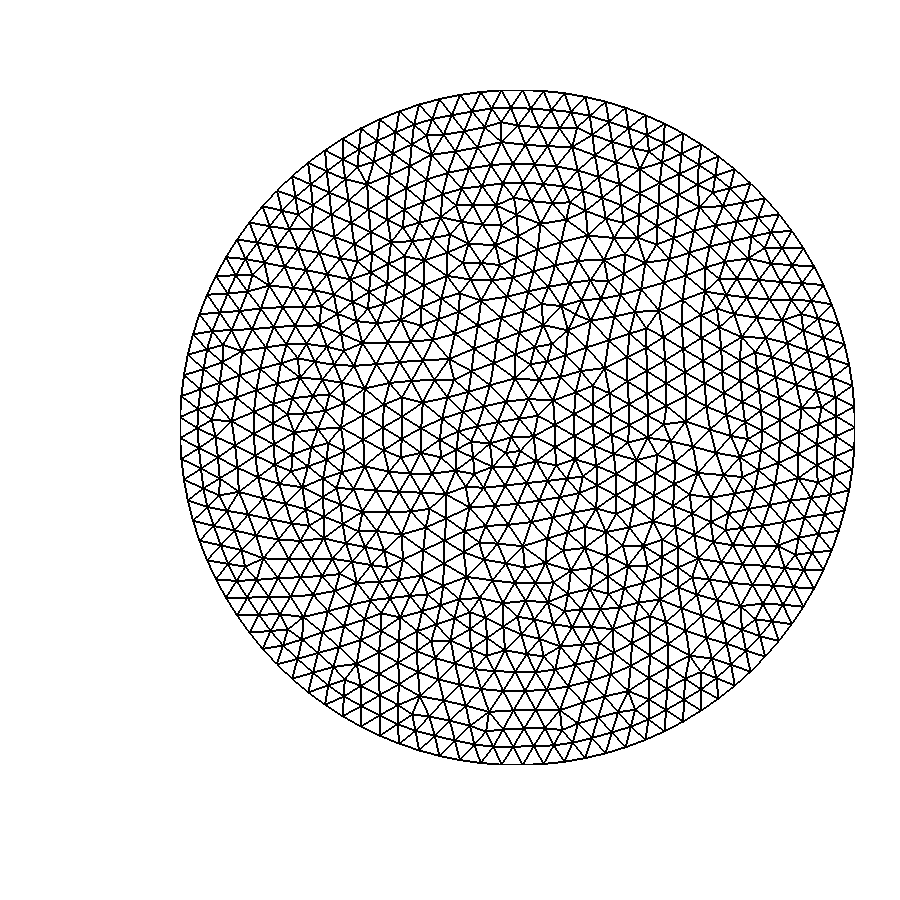
\includegraphics[height=0.13\textheight]{ch18-circle-trelis.png}
\end{center}
\end{frame}

% 29
\begin{frame}{Route E, briefly, and when to use which route}
\label{fr:which}
\scriptsize
\begin{itemize}
  \item \al{MATLAB's PDE Toolbox} (chapter 17, slide 39): \code{pdepoly} for the outline, \textbf{Mesh $\to$ Parameters} for the size, \textbf{Export Mesh}, a \code{fprintf} loop; triangles only, 2D only; the course's plate, the active-tension plate (IBFE/06) and the advection--diffusion plate (IBFE/12) were made this way. Fine if you have MATLAB; gmsh does the same without it.
\end{itemize}
\begin{tabular}{@{}L{0.42\textwidth}L{0.50\textwidth}@{}}
\toprule
you want & route \\
\midrule
a rectangle, box, disc or ball, any size & A: build it in the program (no file to lose; the size follows \code{DX} automatically) \\
a polygon, a tube, a shape you can describe by points and arcs & B: a \code{.geo} script (reproducible; the GUI to look) \\
a shape from a drawing you can trace, with holes & B or C: gmsh with curve loops, or Triangle from a \code{.poly} \\
a body from a scan or a CAD model & D: Coreform Cubit, or gmsh on the STEP/STL \\
hexahedra & D (Cubit), or B with transfinite blocks (\code{tube.geo}) \\
several bodies in one program & any route, one file (or one \code{build\_*} call) per part; chapter 21 \\
\bottomrule
\end{tabular}

\begin{punchbox}
\footnotesize ``In general, the more money spent the easier to use and the more versatile'' (2014) was true of Trelis against gmsh 2. gmsh 4 is easy to script and reads STEP; Cubit still wins for hex meshes and CAD clean-up.
\end{punchbox}
\end{frame}

% 30
\begin{frame}{Element size: five rules the course taught}
\label{fr:fiverules}
\footnotesize
\begin{tabular}{@{}L{0.26\textwidth}L{0.66\textwidth}@{}}
\toprule
source & rule \\
\midrule
2014 Hoover, slide 4 & ``Old: mesh discretizing edge length is $ds = 2\,dx$ (as opposed to $\tfrac12 dx$). New: it seems like $ds = dx$ works better.'' With \code{IB\_POINT\_DENSITY = 2.0} and ``it seems like 1.0 is better.'' \\
2016 gmsh read-me & ``Elements should be close to evenly sized. Average size should equal Cartesian mesh width for fluid solver.'' \\
2016 Trelis notes & ``FE : NS 1:1''; ``wall thickness $4\,dx$.'' \\
2017--2024 homework & ``We want the ratio of the finite element mesh to the Cartesian mesh to be 1:1'': $0.0156$ at $\mathrm{NFINEST} = 128$, with \code{MFAC = 1.0} and \code{IB\_POINT\_DENSITY = 1.0}. \\
2018 Dogwood README (and IBFE/01's) & ``maximum edge size two to four times the fine grid spacing'' ($0.0312$ for the plate), with \code{IB\_POINT\_DENSITY = 2.0}. \\
IBAMR's own examples & \code{MFAC} $1$ to $8$ with \code{IB\_POINT\_DENSITY} $1$ to $4$ (slide \ref{fr:upstream}). \\
\bottomrule
\end{tabular}

\medskip
They look contradictory ($\tfrac12$, $1$, $2$--$4$, up to $8$ grid cells) because they answer different questions: how fine the \emph{elements} must be for the solid mechanics, and how dense the \emph{quadrature points} must be for the fluid--structure coupling. The next slide separates them.
\end{frame}

% 31
\begin{frame}{Element size: what IBAMR does, and the rule that follows}
\label{fr:rules}
\scriptsize
\begin{columns}[T]
\column{0.5\textwidth}
\al{What the mesh is for.} The elements carry the displacement and the stress; their size sets how well the body's shape and strain are resolved. A thin body needs at least two elements across its thickness to bend (the plate has two); a corner needs small elements to stay a corner. This is ordinary finite element judgement and does not involve \code{DX}.

\medskip
\al{What the coupling needs.} Velocity is interpolated to, and force spread from, \emph{quadrature points} of the elements. \code{IB\_point\_density} is the number of those points per fine grid cell that IBAMR aims at; with adaptive quadrature (the default) it raises the rule's order on every element until each has about \code{point\_density} points per cell of its width. Too few points per cell and fluid leaks through the body; the number of \emph{elements} per cell does not matter to the fluid.
\column{0.48\textwidth}
\al{The rule.}
\begin{enumerate}
  \item Make the elements as large as the solid mechanics allows: $\mathrm{ds} \approx \mathrm{DX}$ to $2\,\mathrm{DX}$ for linear elements (\code{TRI3}, \code{TET4}, \code{HEX8}); $2$--$4\,\mathrm{DX}$ for quadratic ones; never larger than half the body's thickness.
  \item Set \code{IB\_point\_density} to $2$ (the upstream default for \code{MFAC = 2}) and raise it to $3$--$4$ if the body leaks or its elements are coarser than $2\,\mathrm{DX}$.
  \item Refine the Cartesian grid, not the mesh, when the flow needs it; refine the mesh when the body's shape does.
\end{enumerate}
So the course's rules were all right for their cases: $1{:}1$ with density $1$ (the homework), $2\,\mathrm{DX}$ with density $2$ (the plate), $8\,\mathrm{DX}$ with density $4$ (upstream ex5's quadratic elements). The one to avoid is the ``$\tfrac12\,dx$'' of 2014: four times the elements for nothing.
\end{columns}
\begin{punchbox}
\footnotesize Cost: the number of quadrature points scales as (body volume) $\times$ \code{point\_density}$^{\mathrm{NDIM}}/\mathrm{DX}^{\mathrm{NDIM}}$, independent of the element size; the FE solve scales with the number of nodes. Coarse elements with dense quadrature are cheap.
\end{punchbox}
\end{frame}

% 32
\begin{frame}[fragile]{Checking a mesh before the first run}
\label{fr:checks}
\footnotesize
\begin{tabular}{@{}L{0.24\textwidth}L{0.68\textwidth}@{}}
\toprule
check & how \\
\midrule
it reads & a ten-line libMesh program, or the example itself with \code{END\_TIME = 0}: \code{mesh.read()} fails fast on a bad extension, a binary file or a missing \code{.node} \\
dimension & the assertion of slide \ref{fr:tworules}; in gmsh, \textbf{Tools $\to$ Statistics} shows how many elements of each dimension \\
element count and type & \code{\$Elements} in the \code{.msh}; the first line of the \code{.ele}; \code{ncdump -h part.e} for Exodus (\code{num\_elem}, \code{num\_el\_blk}, \code{connect1:elem\_type}) \\
orientation & IBAMR's Jacobian check at start-up (slide \ref{fr:tworules}); gmsh: \textbf{Tools $\to$ Options $\to$ Mesh $\to$ Visibility $\to$ Normals} \\
size and position & the node coordinates' range (\code{\$Nodes}) against the box: \code{x\_lo}, \code{x\_up} in \code{CartesianGeometry}; a body that touches a periodic boundary wraps around \\
element size & gmsh \textbf{Statistics} gives the edge-length range; compare with \code{DX} per slide \ref{fr:rules} \\
look at it & gmsh itself; VisIt after \code{gmsh x.msh -save -format vtk -o x.vtk} (or \code{mesh.write("x.e")} from libMesh); the result files' \code{output.ex2} after the first dump \\
\bottomrule
\end{tabular}

\end{frame}

% 32b
\begin{frame}[fragile]{Checking a mesh (2): a ten-line checker}
\label{fr:checks2}
\footnotesize
A ten-line checker, to build like any example (\code{IBAMR::IBAMR2d} brings libMesh):
\begin{lstlisting}[style=cpptiny]
#include <ibtk/IBTKInit.h>
#include <libmesh/mesh.h>
#include <libmesh/mesh_tools.h>
int main(int argc, char* argv[]) { IBTKInit ibtk_init(argc, argv, MPI_COMM_WORLD);
    libMesh::Mesh mesh(ibtk_init.getLibMeshInit().comm(), NDIM); mesh.read(argv[1]); mesh.prepare_for_use();
    mesh.print_info();                                   // dimension, nodes, elements, subdomains, boundary ids
    const auto bb = libMesh::MeshTools::create_bounding_box(mesh);
    libMesh::out << "bounding box " << bb.min() << " to " << bb.max() << std::endl; return 0; }
\end{lstlisting}
\begin{itemize}
  \item \code{print\_info()} lists the dimension, the numbers of nodes and elements, the element types, the subdomains and the boundary ids: everything of the table above except the orientation, which IBAMR tests at start-up.
  \item Build it with the same six-line \code{CMakeLists.txt} as the examples (\code{add\_executable(meshcheck meshcheck.cpp)}); run it as \code{./meshcheck part.msh}.
\end{itemize}
\end{frame}

% 33
\begin{frame}{What was run for this chapter}
\label{fr:run}
\scriptsize
gmsh 4.12.1, Triangle 1.6 and TetGen 1.5.0 (Ubuntu 24.04 packages) in WSL, \code{wsl/final/ch18\_meshtest.sh}; the files are the course's, except \code{triangle.geo} (IBFE/05) and \code{cube.poly} (slide \ref{fr:tetgenrun}):

\begin{tabular}{@{}L{0.20\textwidth}L{0.36\textwidth}L{0.36\textwidth}@{}}
\toprule
input & command & result \\
\midrule
\code{triangle.geo} & \code{gmsh -2 -format msh22} & $759$ nodes, $1404$ \code{TRI3}; MSH 2.2; identical counts to the course's \code{triangle.msh} \\
\code{triangle.geo} & \code{gmsh -2} (no format) & MSH 4.1 (\code{4.1 0 8}): libMesh reads it \\
\code{triangle.geo} & \code{gmsh -2 -format msh22 -bin} & binary (\code{2.2 1 8}): libMesh does not \\
\code{cube.geo} & \code{gmsh -3 -format msh22} & $141$ nodes, $373$ \code{TET4} \\
\code{cone.geo} & \code{gmsh -3 -format msh22} & $648$ nodes; $2460$ \code{TET4} + $1248$ \code{TRI3} + $131$ lines + $6$ points (no physical group) \\
\code{sphere.geo} & \code{gmsh -3 -format msh22} & $60$ nodes; $114$ \code{TET4} + $114$ \code{TRI3} \\
\code{tube.geo} & \code{gmsh tube.geo -0 -format msh22} (the script saves itself) & $593{,}800$ nodes; $579{,}488$ \code{HEX8} + $28{,}112$ \code{QUAD4}; $80$ MB, $1.2$ million lines; $6/5/24$ densities: $2784$ hexahedra \\
\code{IBFE\_Mesh2D\_128.poly} & \code{triangle -pq} & $122$ nodes, $162$ \code{TRI3} \\
\code{cube.poly} & \code{tetgen -pq1.4a0.02 -k} & $75$ nodes, $153$ \code{TET4}, plus a \code{.vtk} \\
\code{plate2.msh}, \code{beam.e}, \code{circle.e} & \code{gmsh -save -format vtk}; VisIt & the pictures of slides \ref{fr:plate2} and \ref{fr:cubit} \\
\bottomrule
\end{tabular}

\medskip
No warnings or errors from gmsh on any of the course's files, gmsh-2 syntax included. The IBAMR-side errors of slide \ref{fr:tworules} are from IBFE/05's README (run on 0.16.0 and 0.19.0).
\end{frame}

% 34
\begin{frame}{What can go wrong}
\label{fr:wrong}
\scriptsize
\begin{tabular}{@{}L{0.40\textwidth}L{0.52\textwidth}@{}}
\toprule
symptom & cause and fix \\
\midrule
\code{Error: Unknown data format for mesh in Gmsh reader.} & a binary \code{.msh}; export ASCII (Version 2 or 4 ASCII) \\
\code{ERROR: Unrecognized file extension} + the format list & the file's extension is not in libMesh's list; rename or convert \\
\code{Failed assertion:}\newline\code{mesh->mesh\_dimension() ==}\newline\code{mesh->spatial\_dimension()} & the file holds only lower-dimensional elements (a \code{Physical Curve} but no \code{Physical Surface}; an STL surface read as a 3D mesh); add the physical group of the body's dimension, or mesh the volume \\
\code{IBAMR requires that the Jacobian of each}\newline\code{element must be positive ...} & clockwise triangles (a clockwise curve loop) or inverted tetrahedra; reverse the loop, \code{ReverseMesh}, or \code{fix\_orientation.py} \\
\code{Error while opening either x.node or x.ele} & TetGen output needs both files next to each other \\
\bottomrule
\end{tabular}

\end{frame}

% 34b
\begin{frame}{What can go wrong (2)}
\label{fr:wrong2}
\scriptsize
\begin{tabular}{@{}L{0.40\textwidth}L{0.52\textwidth}@{}}
\toprule
symptom & cause and fix \\
\midrule
the body is in the wrong place, or huge, or tiny & the mesh is in its own units; scale and move it in the mesher, or register an initial coordinate mapping (chapter 22) \\
fluid passes through the body & too few quadrature points per cell: raise \code{IB\_point\_density}; or the body is thinner than a grid cell \\
the run is far slower than the point example & a mesh much finer than \code{DX} (the ``$\tfrac12 dx$'' rule) or a huge file like the $580$k-hex tube; coarsen, raise the point density \\
gmsh makes a different number of elements than the course file & the 2D algorithm changed between versions (Delaunay 5 vs Frontal-Delaunay 6); set \code{Mesh.Algorithm}; counts within a few per cent are normal \\
the GUI mesh does not update & click \textbf{1D} then \textbf{2D} again (the 2017 and 2016 decks both say so) \\
\code{DefineNumber} parameters share a name & the ONELAB name is the slider's label; give each its own \\
\bottomrule
\end{tabular}

\end{frame}

% 35
\begin{frame}{What the older decks had that is now Part X}
\label{fr:legacy}
\footnotesize
\begin{tabular}{@{}L{0.44\textwidth}L{0.48\textwidth}@{}}
\toprule
2014--2020 & now \\
\midrule
gmsh 2.9.0 (``version ???'' in 2020); \code{Line Loop}, \code{Ruled Surface}; \textbf{File $\to$ Save as} \code{.msh} with no version question & gmsh 4; \code{Curve Loop}, \code{Surface} (the old names still work); \textbf{Export} with the MSH version dialog: Version 2 ASCII \\
Trelis and Bolt (csimsoft; a shared floating licence on the lab's Windows machine; \code{csimsoft.com} links) & Coreform Cubit (\url{https://coreform.com}); the vendor PDF linked, not copied \\
Meshmixer for STL clean-up & discontinued (2021); Blender's remesh, MeshLab \\
\code{TET8}, \code{HEX6}, ``Hexagonal'' & \code{TET10}, \code{PRISM6}, hexahedral (slide \ref{fr:elemtypes}) \\
\code{Mesh mesh(NDIM); TetGenIO TETGEN(mesh);}\newline\code{TETGEN.read(}\newline\code{"Jellyfish\_IBFE\_Mesh3D.ele");} & \code{Mesh mesh(init.comm(), NDIM);}\newline\code{mesh.read("x.ele");} (the jellyfish file never shipped) \\
``modify the \code{main.C} file to read in the mesh'' & \code{MESH\_FILENAME} in the input file \\
\code{MFAC = 1.0} ``to update to 1:1'' for a read-in mesh & no effect; the element size is in the file; \code{IB\_point\_density} is the knob \\
the meshing read-me's forwarded IT e-mail about the licence server & not reproduced (privacy); the licence is history \\
\bottomrule
\end{tabular}

\end{frame}

% 36
\begin{frame}{Exercises}
\label{fr:exercises}
\footnotesize
\begin{enumerate}
  \item Make the IBFE/01 plate ($1.0\times0.0312$) in gmsh with \code{lc = 0.03}, export MSH 2.2, and run \code{MOTION = "FULL"} with it. Compare the centre positions with chapter 17's table; then halve \code{lc} and compare again.
  \item Take \code{triangle.geo}, make the curve loop clockwise, mesh, and run IBFE/05 until it stops. Fix the file three ways (the loop, \code{ReverseMesh}, \code{fix\_orientation.py}) and check that all three meshes are the same.
  \item Write the plate-with-a-hole \code{.poly} of slide \ref{fr:holes}, mesh it with \code{triangle -pqa0.0005}, convert the \code{.node}/\code{.ele} pair to MSH 2.2 with a script of your own, and run it in IBFE/01's program. What does the hole do to the FULL motion?
  \item Finish Battista's tube: add the surface loop, volume and physical volume to the \code{.geo} he built, mesh it in 3D, and read it with the checker of slide \ref{fr:checks}. How many tetrahedra at \code{ds = L/100}?
  \item Run \code{tube.geo} at the three densities $6/5/24$, $8/10/60$ and the original $15/20/200$; tabulate nodes, hexahedra, file size and the time gmsh takes. Which would you use at $\mathrm{DX} = 1/16$?
  \item Rebuild IBFE/10's plate ($0.125\times2\times2$, about $3\,\mathrm{DX}$ elements) from a \code{.geo} of your own by extruding a square, and compare the node count with \code{plate2.msh}'s $3{,}386$.
  \item Build the same plate inside the program with \code{build\_cube} and \code{MFAC = 3}, run both for $0.5$ s, and compare the tether force lines of the two runs.
\end{enumerate}
\end{frame}

% 37
\begin{frame}{Rules of thumb}
\label{fr:thumb}
\small
\begin{itemize}
  \item A \code{.geo} script beats the mouse: reproducible, diffable, and it is what the GUI writes anyway.
  \item Counter-clockwise loops; a \code{Physical Surface} or \code{Physical Volume}; export MSH 2.2 ASCII.
  \item Elements as large as the solid allows ($\mathrm{DX}$ to $2\,\mathrm{DX}$ for linear elements, two across any thickness); \code{IB\_point\_density} $2$, more if it leaks.
  \item \code{MFAC} and \code{ELEM\_TYPE} are for meshes built in the program; a file brings its own size and type.
  \item Check dimension, counts, bounding box and orientation before the first run; IBAMR's own checks catch the last two.
  \item TetGen output is a pair of files and 3D only; Triangle output needs a conversion for 2D, or use gmsh.
  \item Exodus blocks and gmsh physical groups become subdomains: name them, you will want them in chapter 21.
  \item Keep the mesher's input next to the mesh in the example folder, and make sure it is the input that made the mesh.
\end{itemize}
\end{frame}

% 38
\begin{frame}{Summary}
\label{fr:summary}
\footnotesize
\begin{enumerate}
  \item IBFE takes a mesh of the program's dimension, of one of libMesh's element types, with positive Jacobians, placed and scaled in the simulation's units, from a file whose extension picks the reader, or built in the program with libMesh's generators.
  \item gmsh makes 2D and 3D meshes from a script or by mouse; MSH 2.2 or 4.1 ASCII, never binary; a counter-clockwise loop and a physical group are the two rules; physical names become subdomain and side-set names.
  \item Triangle and TetGen mesh a \code{.poly} file of nodes, segments or facets, holes and regions; TetGen's \code{.node}/\code{.ele} pair reads directly in 3D.
  \item CAD goes through Coreform Cubit (Trelis's successor) or gmsh to ExodusII or MSH; Exodus blocks become subdomains.
  \item The element-size rules of ten years agree once the elements (solid resolution) and the quadrature points (\code{IB\_point\_density}, the coupling) are separated: elements of $\mathrm{DX}$ to $2\,\mathrm{DX}$, points $2$ per cell, more points before smaller elements.
  \item Every command here was run today on the course's own files; the counts are on slide \ref{fr:run}, the errors on slides \ref{fr:tworules} and \ref{fr:wrong}.
\end{enumerate}
\begin{homebox}
\footnotesize Chapter 19 writes the stress functions; chapter 21 gives parts of a mesh different materials through the subdomain ids made here; chapter 22 moves a mesh into place with a coordinate mapping.
\end{homebox}
\end{frame}

% 39
\begin{frame}{Recordings and links (listed, not incorporated)}
\label{fr:videos}
\small
\begin{itemize}
  \item The lab's July 2022 Coreform Cubit tutorial recording (private Drive; listed in chapter 0.1).
  \item The 2016 gmsh read-me's links: the Fluidity project's gmsh tutorial (\url{https://github.com/FluidityProject/fluidity/wiki/Gmsh-tutorial}) and two YouTube gmsh tutorials (``part 1'' \code{xL2LmDsDLYw}, ``part 3'' \code{laKHzos3EbU}); gmsh's own documentation at \url{https://gmsh.info/doc/texinfo/gmsh.html}.
  \item csimsoft's Trelis tutorials and videos (\code{csimsoft.com/tutorialsTrelis}, dead) and the \emph{Getting Started with Trelis} PDF (2014): see \url{https://coreform.com} for their successors.
  \item Triangle: \url{https://www.cs.cmu.edu/~quake/triangle.html}; TetGen: \url{https://wias-berlin.de/software/tetgen/}.
\end{itemize}
\end{frame}

% 40
\begin{frame}{References and credits}
\label{fr:refs}
\scriptsize
\begin{itemize}
  \item C. Geuzaine and J.-F. Remacle, \emph{Gmsh: a three-dimensional finite element mesh generator with built-in pre- and post-processing facilities}, Int.\ J.\ Numer.\ Meth.\ Engng 79 (2009) 1309--1331.
  \item J. R. Shewchuk, \emph{Triangle: engineering a 2D quality mesh generator and Delaunay triangulator}, in \emph{Applied Computational Geometry}, LNCS 1148 (1996) 203--222. H. Si, \emph{TetGen, a Delaunay-based quality tetrahedral mesh generator}, ACM Trans.\ Math.\ Softw.\ 41 (2015) 11.
  \item libMesh 1.7.8: \code{include/libmesh/mesh\_generation.h}, \code{src/mesh/gmsh\_io.C}, \code{tetgen\_io.C}, \code{exodusII\_io.C}, \code{namebased\_io.C}; \url{https://libmesh.github.io}. IBAMR 0.19.0: \code{src/IB/FEMechanicsBase.cpp} (the Jacobian check), \code{examples/IBFE/explicit/ex0}--\code{ex11}.
  \item The examples of this series: IBFE/05 gmsh triangle (\code{triangle.geo}, \code{triangle.msh}, \code{fix\_orientation.py}), IBFE/10 (\code{plate2.msh}), IBFE/08 (\code{beam.e}, \code{circle.e}), IBFE/01 \code{extras/} (\code{Beam\_IBFE\_Mesh2D.m}, \code{.poly}); \code{wsl/final/ch18\_meshtest.sh}, \code{ch18\_render.sh}.
  \item Sources: Alex Hoover, \emph{2-IBFE Tutorial: Creating your mesh} (2014--2017); \emph{2.1 - IBFE Tutorial: Make your own mesh and move it!} (2017; MATH 769 2018; lab 2020--2024); Julian Wag, \emph{Using gmsh to make 2D meshes from scratch} (2016; screenshots reproduced with credit); Nick Battista, \emph{How To Make Simple Geometries in Gmsh} (24 September 2014; cited); the meshing, gmsh and Trelis read-mes (2015--2017) and the 2016 Trelis notes; the \code{cube}, \code{cone}, \code{sphere} and \code{tube} \code{.geo} samples of the meshing folder; \emph{5-IBFE Lecture: Plans for June} (2020).
\end{itemize}
\end{frame}

\end{document}
